\customlink{Applied_rock_(environmental)_magnetism}
\chapter{Applied rock (environmental) magnetism}

\noindent
BACKGROUND: read Maher and Thompson (1999), chapter 1; \nocite{maher99}
Evans and Heller (2003), chapter 4. \nocite{evans03}

\vskip 24pt



There is a lively field within rock magnetism that exploits the dependence of  rock magnetic parameters on concentration, grain size and mineralogy for gleaning information about past (and present) environments.  Examples of applied rock magnetism 
\index{environmental magnetism}
 {\it (environmental magnetism)} run from detection of industrial pollution to characterizing changes across major  climatic events    In this chapter we will review the basic tool-kit used by environmental magnetists and illustrate various applications with examples.   

Applied rock magnetism relies on imaging techniques and magnetic measurements.  Images come from optical microscopes, magnetic force microscopes,  scanning electron and transmission electron microscopes   using magnetic separates, polished sections or thin sections.   Magnetic measurements include magnetic susceptibility,  magnetic remanence  and hysteresis, all as a function of temperature.  All of these measurements can also be done as a function of orientation, but orientation is not  usually important  in environmental applications;   anisotropy of rock magnetic measurements will be the topic of a later chapter.    A list of the most frequently used parameters is included in Table~\ref{tab:params}.  


\section{Images}


Images of magnetic phases are used to shed light on  the origin of the magnetic phases.    Scanning electron microscope images of igneous (Figure~\ref{fig:images}a), detrital or aeolian (Figure~\ref{fig:images}b), authigenic (Figure~\ref{fig:images}c), biogenic (Chapter 6),  anthropogenic (Figure~\ref{fig:images}d)  and cosmic (Figure~\ref{fig:images}e) sources all have distinctive ear-marks, so actually looking at the particles in question can provide invaluable information.



\begin{figure}[h!tb]
%\epsfxsize 14.5cm
%\centering \epsffile{EPSfiles/images.eps}
\centering  \includegraphics[width=14.5 cm]{EPSfiles/images.eps}
\caption{Images of various magnetic phases.  a) 300 $\mu$m titanomagnetite grain of igneous origin showing high temperature exsolution lamellae  [Photo from R. Reynolds in Maher and Thompson, 1999.]. b) Detrital and aeolian (titano)magnetites from Chinese Loess.  [Photo from Maher and Thompson, 1999.]  c) Hematite rosettes on a smectite surface.  [Photo from Reynolds et al., 1985.]  d) Backscatter SEM image of fly-ash spherule. [Photo of J. Matzka, in Maher and Thompson, 1999.]  The bright grains are iron rich particles embedded in a silicate matrix.  e) Silicate spherule with dendrites of Fe-rich material of cosmic origin, showing characteristic pitting of the surface. [Photo from M. Hounslow in Maher and Thompson, 1999.]   }
\label{fig:images}
\end{figure}
 \nocite{maher99}
\nocite{reynolds85}

\begin{table}
\caption{Summary of environmental magnetic parameters.}
\label{tab:params}
\begin{tabular}{llll}
\hline
Parameter name & Symbol & Units & Section\\
\hline
Critical temperatures:\\
\hskip 1em median destructive temperature& MDT & $^{\circ}$C or K & \ref{sect:crittemp}\\
\hskip 1em Curie (N\'eel) Temperature & $T_c$ & $^{\circ}$C or K & \ref{sect:ferro}, \ref{sect:crittemp}\\\
\hskip 1em Hopkinson Effect & $T_h$ & $^{\circ}$C or K & \ref{sect:crittemp}\\
\hskip 1em Verwey transition & $T_v$ & $^{\circ}$C or K & \ref{sect:K1},\ref{sect:titano}\\
\hskip 1em Morin transition & $T_m$ & $^{\circ}$C or K & \ref{sect:hemo}\\
\hskip 1em Pyrrhotite transition&$T_p$& $^{\circ}$C or K & \ref{sect:pyrrho}\\
\hline
Magnetic susceptibility: \\
\hskip 1em \hskip 1em volume normalized & $\chi$ &dimensionless &\ref{sect:mag}\\
\hskip 1em mass normalized & $\kappa$ & m$^3$kg$^{-1}$&\ref{sect:mag}\\
\hskip 1em low field (initial) & $\chi_{lf}$\& \ref{sect:chi}\
\hskip 1em high field & $\chi_{hf}$&\ref{sect:chi},\ref{sect:hyst}\\
\hskip 1em frequency dependent & $\chi_{fd}$&\ref{sect:chifd}\\
\hline
Magnetization: \\
\hskip 1em volume normalized &$M$ &Am$^{-1}$&\ref{sect:mag}\\
\hskip 1em mass normalized &$\Omega$ & Am$^2$kg$^{-1}$&\ref{sect:mag}\\
\hskip 1em saturation & $M_s$ &&\ref{sect:para},\ref{app:hyst}\\
\hskip 1em saturation remanence &$M_{r}$ or sIRM&& \ref{sect:uniaxial},\ref{sect:irm},\ref{app:hyst}\\
\hskip 1em isothermal remanence & IRM&& \ref{sect:uniaxial},\ref{sect:irm} \\

\hskip 1em anhysteretic remanence & ARM&&\ref{sect:arm}\\
\hskip 1em partial anhysteretic remanence & pARM&&\ref{sect:arm}\\
\hskip 1em ARM susceptibility & $\chi_{ARM}$&dimensionless&8\\
\hline
Critical fields:\\
\hskip 1em Coercivity & $H_{c}$ or $\mu_oH_{c}$  & Am$^{-1}$ or T & \ref{sect:K1},\ref{sect:uniaxial},\ref{app:hyst}\\
\hskip 1em Coercivity of remanence & $H_{cr}$ or $\mu_oH_{cr}$  & Am$^{-1}$ or T & \ref{sect:uniaxial},7,\ref{app:hyst}\\
\hskip 1em median destructive field& MDF & Am$^{-1}$ or T& \ref{sect:crittemp}\\
\hline
Ratios:\\
\hskip 1em Squareness & $M_r/M_s$ && \ref{sect:uniaxial}\\
 & $H_{cr}/H_{c}$ &&\ref{sect:day}\\
\hskip 1em S-ratio & IRM$_x$/$M_r$ & & \ref{sect:ratios}\\
\hskip 1em HIRM  & $M_r$ - IRM$_x$ & &\ref{sect:ratios}\\
\hskip 1em &$M_r$/$\chi$&&\ref{sect:ratios}\\
& $\chi_{ARM}/\chi$&&\ref{sect:ratios}\\
& ARM/$M_r$&&\ref{sect:ratios}\\
\hskip 1em K\"onigsberger ratios& $Q_n, Q_t$  &dimensionless&\ref{sect:ratios}\\
\hskip 1em $\delta-\delta$ & $\delta_{FC}/\delta_{ZFC}$ &dimensionless&\ref{sect:delta}\\
\hskip 1em  IRM crossover&$R_{x}$ &dimensionless&\ref{sect:crossover}\\
\hline
\end{tabular}
\end{table}
\nocite{koenigsberger38}




\section{Critical temperatures}
\label{sect:crittemp}

In Table~\ref{tab:params} we list  several 
\index{critical temperatures}
{\it critical temperatures}  useful for characterizing the magnetic mineralogy of specimens  
that are observed in  magnetic systems.  The 
\index{Curie temperature}
\index{N\'eel!temperature}
Curie (and N\'eel) temperatures above which spontaneous magnetization  ceases, the 
\index{Verwey transition}
\index{Morin transition}
Verwey and    Morin transitions in magnetite and hematite respectively and the 
\index{pyrrhotite!transition}
pyrrhotite transition at which the magnetic  anisotropy energies change character resulting in an observable effect in the magnetization  were all encountered  in previous chapters.  However, there are several critical temperatures  that are new, or require additional clarification.   The so-called
\index{Hopkinson effect}
 {\it Hopkinson effect}  listed in Table~\ref{tab:params}  is discussed in Section~\ref{sect:chiT} under magnetic susceptibility measurements.    The 
 \index{median destructive!temperature}
 {\it median destructive temperature} is simply the temperature at which 50\% of the NRM is destroyed when a specimen is heated to that temperature and cooled in zero field.  It is a measure of stability, only rarely used and only mentioned here for completeness.    [An analogous parameter for stability against alternating fields is the 
 \index{median destructive!field}
 {\it median destructive field}  (MDF), which is the alternating field required to reduce a remanence to 50\% of its initial value.]
 



Although we defined the Curie temperature in Chapter 3, we did not really describe how the measurements were made or how the temperature can be estimated.   The principles are illustrated in Figure~\ref{fig:curiebalance}.  A specimen is placed near the pole pieces of a strong electromagnet.   The field gradient will pull a magnetic specimen in.  A pick-up coil counteracts this force with  a restoring force of equal magnitude.  The current required to keep the specimen stationary is proportional to the magnetization.    A thermocouple monitors the temperature as the specimen heats in a water cooled oven.  Both the output of the pickup coil and the thermocouple can be put into a computer to make a graph of saturation magnetization versus temperature an example of which is shown as the solid line in Figure~\ref{fig:curie1}a.  

 \begin{figure}[htb]
%\epsfxsize 12.5cm
%\centering \epsffile{EPSfiles/curiebalance.eps}
\centering  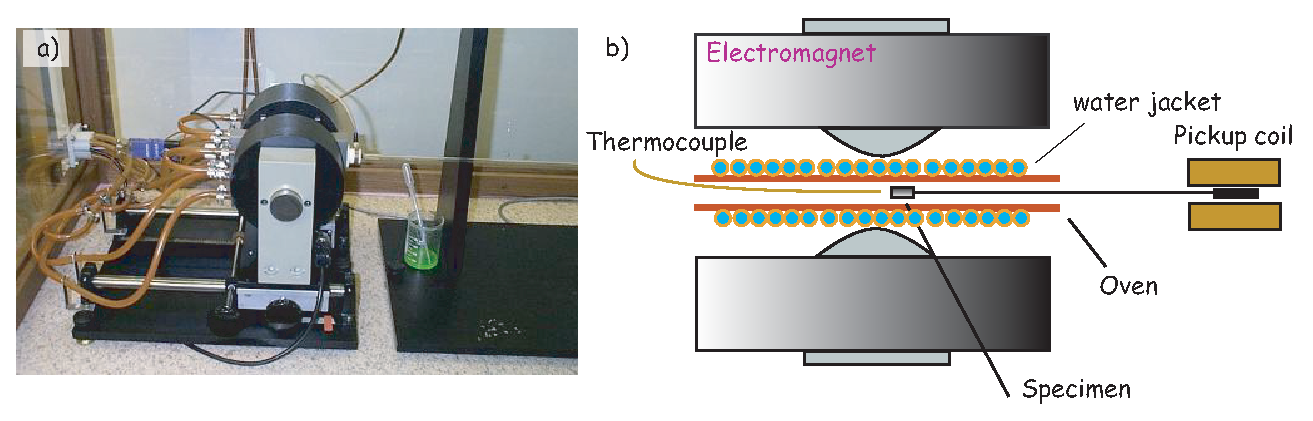
\includegraphics[width=12.5 cm]{EPSfiles/curiebalance.eps}
\caption{a) Translation curie balance in the Scripps Laboratory.  b) Schematic drawing of the key elements of a) (top view). }
\label{fig:curiebalance}
\end{figure}



Estimating the 
\index{Curie temperature!estimation}%
Curie temperature is not as simple as it seems at first
glance.  \nocite{gromme69}
\index{Gromm\'e, C.S.}
Gromm\'e et al. (1969)  used the  
the intersection point of the two tangents to the
thermomagnetic curve that bounds the Curie temperature, as shown in the inset to 
Figure~\ref{fig:curie1}a.  The 
\index{Curie temperature!estimation!intersecting tangents method}
{\it intersecting tangents method} is 
straightforward to do by hand, but is rather subjective and 
is difficult to automate. 
\index{Curie temperature!estimation!Moskowitz method}
\nocite{moskowitz81}
\index{Moskowitz, B.M.}
Moskowitz (1981) applied a method based on statistical physics for extrapolating
the ferromagnetic behavior expected from experimental data
 through the Curie temperature to determine the point at which the
ferromagnetic contribution reaches zero.  


\begin{figure}[htb]
%\epsfxsize 14cm
%\centering \epsffile{EPSfiles/curie1.eps}
\centering  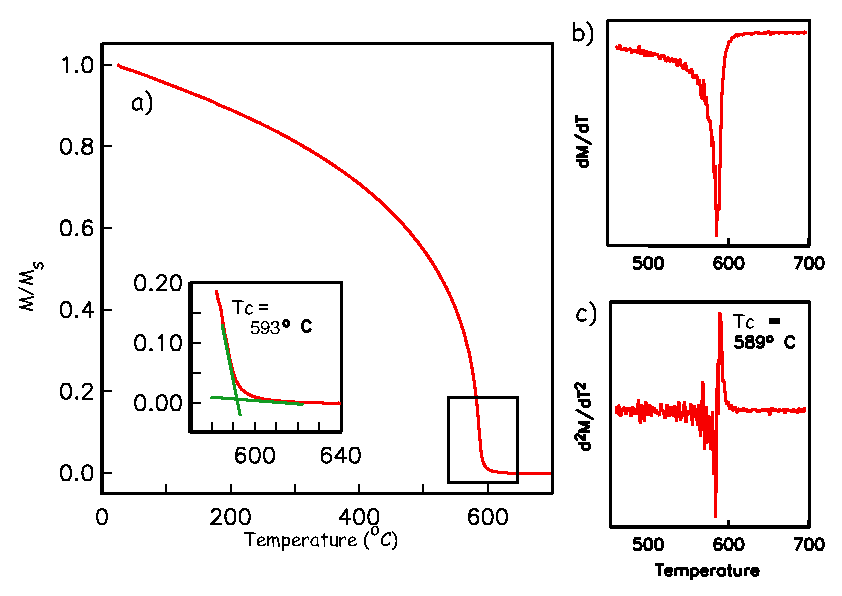
\includegraphics[width=14 cm]{EPSfiles/curie1.eps}
\caption{a) $M_s-T$  data for magnetite.  Inset illustrates intersecting tangent method of Curie temperature estimation.  b) Data from a) differentiated once.  c) Data from a) differentiated twice.  Peak shows temperature of maximum curvature, interpreted as the Curie temperature for this specimen. }
\label{fig:curie1}
\end{figure}


A third method
 for estimating Curie temperatures from thermomagnetic data, 
 the
 \index{Curie temperature!estimation!differential method}
  {\it differential method} of 
  \index{Tauxe, L.}
  Tauxe (1998),   \nocite{tauxe98}
seeks the maximum curvature in the thermomagnetic
curve.
 This method is shown in Figure~\ref{fig:curie1}b,c. First, we calculate the
derivative ($dM/dT$) of the data in Figure~\ref{fig:curie1}a (see
Figure~\ref{fig:curie1}b). Then, these data are differentiated once again to
produce $d^2M/dT^2$ (Figure~\ref{fig:curie1}c).  The maximum in the second derivative
occurs at the point of maximum curvature in the thermomagnetic curve and is a
reasonable estimate of the Curie temperature.


The principal drawback of the
differential method of Curie temperature estimation
 is  that noise in the data is greatly
amplified by differentiation, which  makes identification of the Curie temperature
difficult. 
These drawbacks  can often be
overcome  by smoothing the data either by calculating three or more point running
means, or using some filter either by Fourier methods or in the
temperature domain.

  There are a host of other measurements of remanent magnetization as a function of  temperature.  These can contribute significantly to the discussion of degree of alteration, degree of particle interaction and  grain size of the magnetic phases in  a specimen.    A complete discussion of these are beyond the scope of this chapter, but the student should be aware of the rich possibilities of low and high temperature measurements of remanence.  For interesting examples,  peruse the various issues of the IRM Quarterly at: \href{http://www.irm.umn.edu/IRM/quarterly.html}{http://www.irm.umn.edu/IRM/quarterly.html}.  

\vskip -12pt
\index{magnetic!susceptibility}
\section{Magnetic susceptibility}



We first encountered the  concept of magnetic susceptibility  in Chapter  1  and again in more detail  in Chapters 3 and 5. 
We defined it as the ratio of  the  induced magnetization to an inducing magnetic field or $M_I/H$.  Because everything in a rock or mineral separate contributes to the magnetic susceptibility, it can be a fertile source of information on the composition of the sample.  [For the same reasons, it can also be somewhat nightmarish to interpret on its own.]   It is quick and easy to measure both in the field and in the laboratory;  hence, magnetic susceptibility is used in  a variety of ways in applied rock magnetism, including lithologic correlation,   magnetic fabric,  magnetic grain size/domain state, mineralogy and so on.  

\begin{figure}[htb]
%\epsfxsize 13cm
%\centering \epsffile{EPSfiles/kappa.eps}
\centering  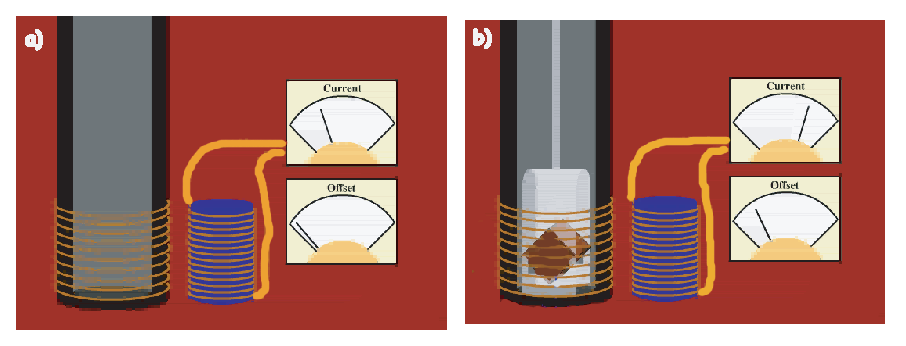
\includegraphics[width=13 cm]{EPSfiles/kappa.eps}
\caption{Measuring magnetic susceptibility.  a)  An alternating current applied in the coil on the right induces a current in the left-hand coil.  This induces a magnetization in the specimen shown in b), which in turn offsets the current in the coil to the right.  The offset is proportional to the magnetic susceptibility of the specimen. [Modified from Genevieve Tauxe animation at: {http://magician.ucsd.edu/Lab\_tour/movs/isosuscp.mov}.] }

\label{fig:kappa}
\end{figure}
%
%
%
It is worth thinking briefly about what controls magnetic susceptibility and what the data might mean.  At an atomic level, magnetic susceptibility results from the response of electronic orbits and/or unpaired spins to an applied field (Chapter 3).    The diamagnetic response (orbits) is extremely weak and unless a specimen, e.g., from some ocean sediments,  is nearly pure carbonate or quartz, it can be neglected.  The paramagnetic response of, say, biotite, is much stronger, but if there is any appreciable ferromagnetic material in the specimen, the response will be dominated by that.    In highly magnetic minerals such as  magnetite, the susceptibility is dominated by the shape anisotropy.   For a uniformly magnetized  particle (e.g., small SD magnetite), the maximum susceptibility is at a high angle to the easy axis, because the moments are already at saturation along the easy direction.  So we have the somewhat paradoxical result that uniformly magnetized particles have maximum susceptibilities along the short axis of elongate grains.   For  vortex remanent state, or multi-domain particles and perhaps for strongly flowered grains, this would not be the case and the maximum susceptibility is along the particle length. Another perhaps non-intuitive behavior is for superparamagnetic particles whose response is quite large.  We learned in Chapter 7 that it can be as much as 27 times  larger than a single domain particle of the same size!   Chains of particles may also have magnetic responses arising from  inter-particle interaction.   Therefore, although magnetic susceptibility is quick to measure, its interpretation may not be straight-forward.   


\index{magnetic!susceptibility!measurement of }
\subsection{Measurement of magnetic susceptibility}

Many laboratories use equipment that works on the principle illustrated in Figure~\ref{fig:kappa} whereby an alternating current is driven through the coil on the right inducing a current in the coil on the left.  This alternating current generates a small alternating field (generally less than 1 mT) along the axis of the coil.  When a specimen is placed in the coil (Figure~\ref{fig:kappa}b), the alternating current induces an alternating magnetic field in the specimen.  This causes an offset in the alternating current in the coil on the right which is proportional to the induced magnetization.  After calibration, this offset can then be cast in terms of magnetic susceptibility.   If the specimen is placed in the solenoid in different orientations  the anisotropy of the magnetic susceptibility can be determined, a topic which we defer to Chapter  13.  

\begin{figure}[htb]
%\epsfxsize 14cm
%\centering \epsffile{EPSfiles/chiT.eps}
\centering  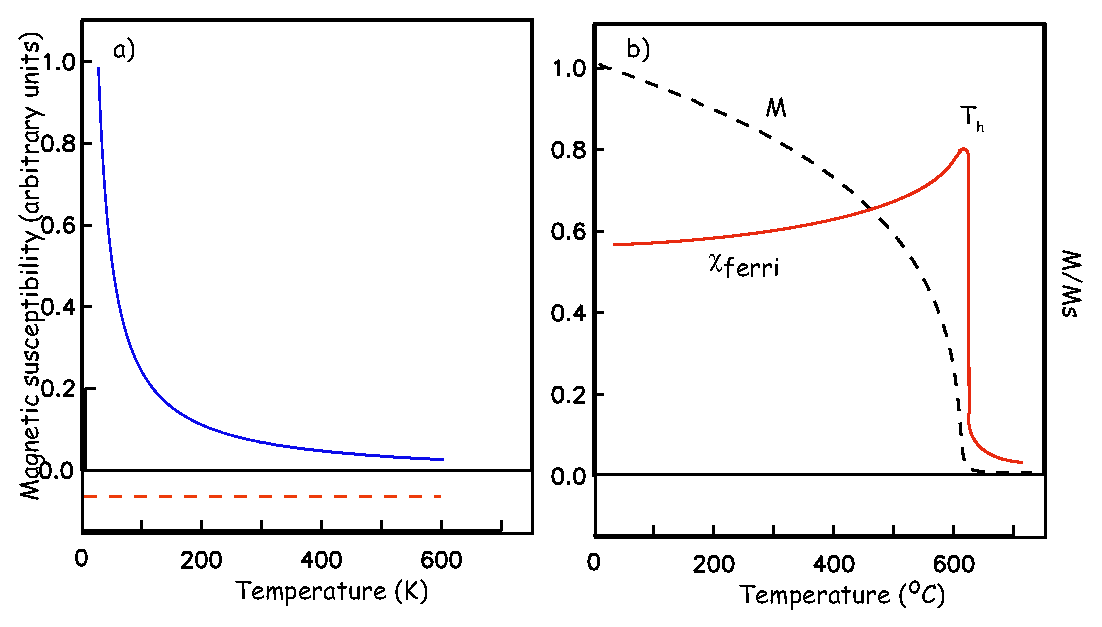
\includegraphics[width=14 cm]{EPSfiles/chiT.eps}
\caption{a) Schematic drawings of paramagnetic (solid line) and diamagnetic (dashed line) magnetic susceptibility as a function of temperature.  b) Behavior of ferromagnetic susceptibility (solid line) as the material approaches its Curie temperature ($M_s-T$ data shown as dashed line).  }
\label{fig:chiT}
\end{figure}

\subsection{Temperature dependence}
\label{sect:chiT}

 Susceptibility can be measured as a function of temperature by placing the specimen in a heating coil (see examples in Figure~\ref{fig:chiT}).  
 We know from Chapter 3 that diamagnetism is negative and  independent of temperature (dashed line in Figure~\ref{fig:chiT}a) and that  paramagnetism is inversely proportional to temperature (solid line in Figure~\ref{fig:chiT}a).      There is a difference of a factor of $\ln(C\tau)$ or about 27 between the superparamagnetic and the stable single domain magnetic susceptibility for a given grain.  This means that as the blocking temperatures of the magnetic grains in a particular specimen are reached, the susceptibility of the grain will increase by this factor until the Curie temperature is reached, at which point only paramagnetic susceptibility is exhibited and the susceptibility will drop inversely with temperature (solid line in  Figure~\ref{fig:chiT}b).    An SP peak in susceptibility below the Curie temperarure could explain the so-called 
 \index{Hopkinson effect}
 {\it Hopkinson effect}  which is a peak in magnetic susceptibility associated with the Curie temperature.   The Hopkinson effect is frequently used to approximate Curie temperatures but may  actually be related to unblocking in some specimens.  



\begin{figure}[htb]
%\epsfxsize 14.5cm
%\centering \epsffile{EPSfiles/chifd.eps}
\centering  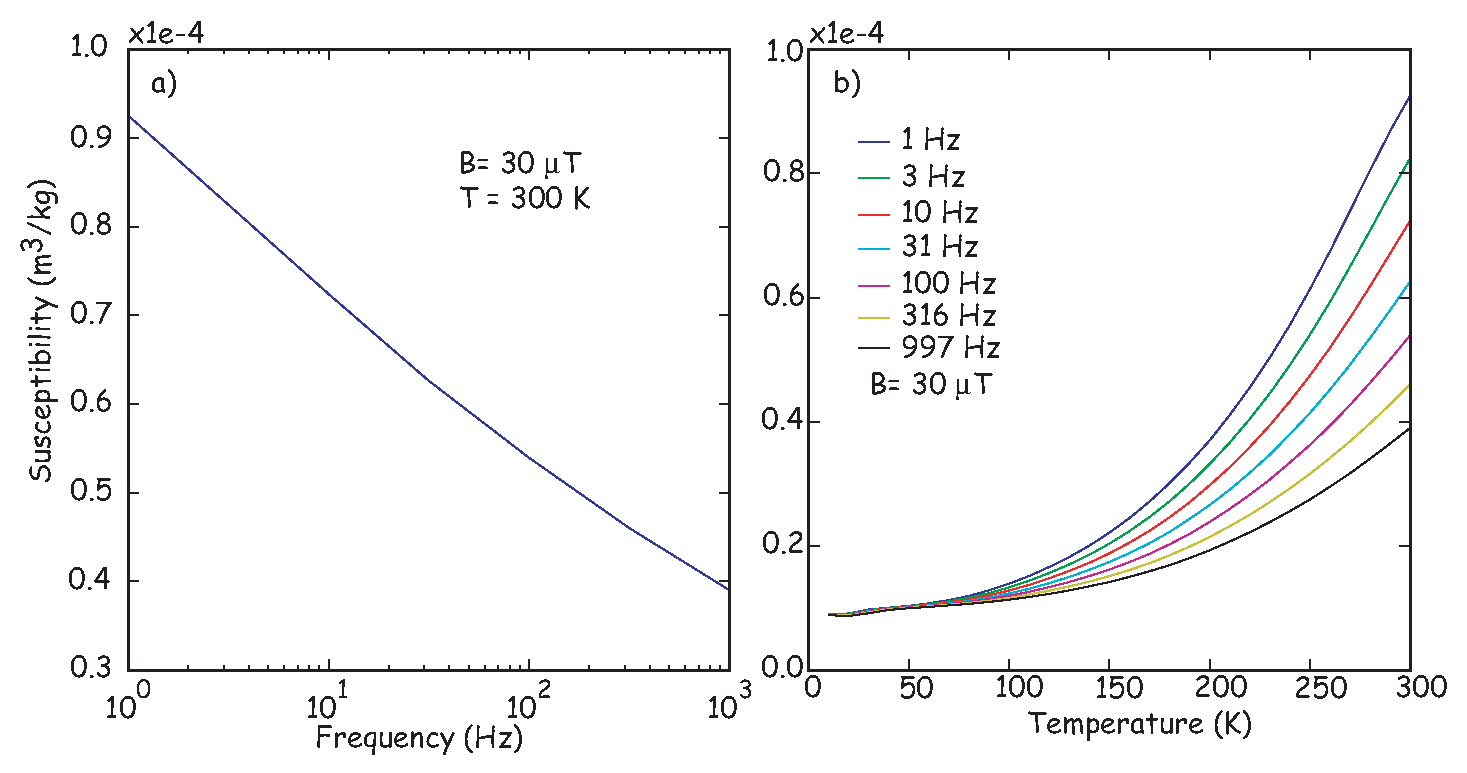
\includegraphics[width=14.5 cm]{EPSfiles/chifd.eps}
\caption{a)  Magnetic susceptibility as a function of frequency.  The decrease in frequency dependence of susceptibility  with increasing frequency is caused by the superparamagnetic particles in the specimen.  b)   Plot showing temperature and frequency dependence of the same specimen as in a).  [Data from Tiva Canyon Tuff, Carter-Stiglitz et al. 2006.] }
\label{fig:chifd}
\end{figure}
 \nocite{carterstiglitz06}

 
 \index{magnetic!susceptibility!frequency dependence}
\subsection{Frequency dependence}  
\label{sect:chifd}

 Susceptibility can also be measured as a function frequency of the applied oscillating field.   
 \index{superparamagnetism}
Superparamagnetic  behavior depends on the time scale of observation (the choice of $\tau$) so grains may behave superparamagnetically at one frequency, but not at another.   Frequency dependent susceptibility $\chi_{fd}$ can therefore  be used to constrain grain size/ domain state of magnetic materials.   We illustrate this effect in Figure~\ref{fig:chifd} which shows data gathered at the Institute for Rock Magnetism (IRM) on samples of the Tiva Canyon Tuff which are well known for their superparamagnetic/single domain grain size range 
\index{Schlinger, C.M.}   \nocite{schlinger91}
(e.g., Schlinger et al., 1991). 

In Figure~\ref{fig:chifd}a we show measurements made at room temperature. Because of the far greater magnetic susceptibility of superparamagnetic particles, $\chi$ drops with the loss of SP behavior.  Magnetic grains that act superparamagnetically at 1 Hz, may behave as stable single domains at higher frequencies (remember that SP behavior depends on time scale of observation), hence the loss of magnetic susceptibility with increasing frequency in the Tiva Canyon Tuff specimens.    While the magnetization drops with increasing frequency, it can rise with increasing temperature as described in Section~\ref{sect:chiT}.    This behavior is shown in Figure~\ref{fig:chifd}b.  

\begin{figure}[htb]
%\epsfxsize 12cm
%\centering \epsffile{EPSfiles/chimap.eps}
\centering  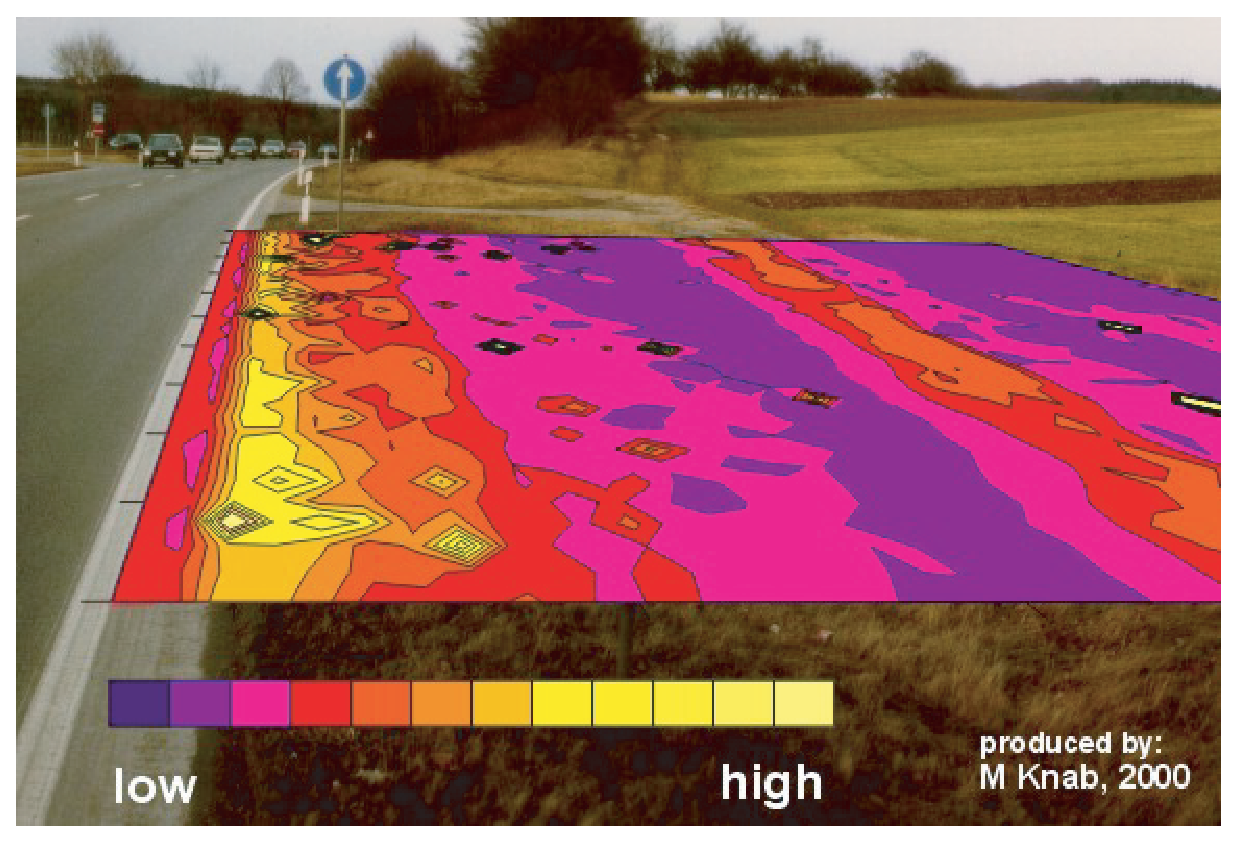
\includegraphics[width=12 cm]{EPSfiles/chimap.eps}
\caption{Map of magnetic susceptibility as a function of distance from the road.  [Data from Hoffmann et al., 1999;  Figure of M. Knab.]}
\label{fig:chimap}
\end{figure}  \nocite{hoffmann99}

\subsection{Outcrop measurements}

Although most laboratories make magnetic susceptibility measurements on small specimens, it is also possible to make measurements on core sections or even at the outcrop.   The latter can be done with hand held susceptometers various shapes and sizes, depending on the application.      We show a map made with a field device  in Figure~\ref{fig:chimap}.  Magnetic susceptibility is enhanced where magnetite spheres produced in the combustion of petroleum products are present as pollutants in dust particles.  Therefore, magnetic susceptibility can be used as a tracer of industrial pollution (see, e.g., 
\index{Petrovsky, E.}
Petrovsky et al. 2000).       \nocite{petrovsky00}

\section{Magnetization}
\label{sect:rmrm}


Table~\ref{tab:params} lists various magnetizations that are useful in applied rock magnetism.  These were all introduced  in previous chapters but several deserve additional discussion.  We  will discuss the hysteresis parameters, $M_r$ and $M_s$ together with their critical field counterparts $H_c$ and $H_{cr}$ in  Section~\ref{sect:hyst}.   In this section we will flesh out our understanding of IRM with particular attention to its uses in applied rock magnetism.  

\begin{figure}[htb]
%\epsfxsize 14cm
%\centering \epsffile{EPSfiles/crossover.eps}
\centering  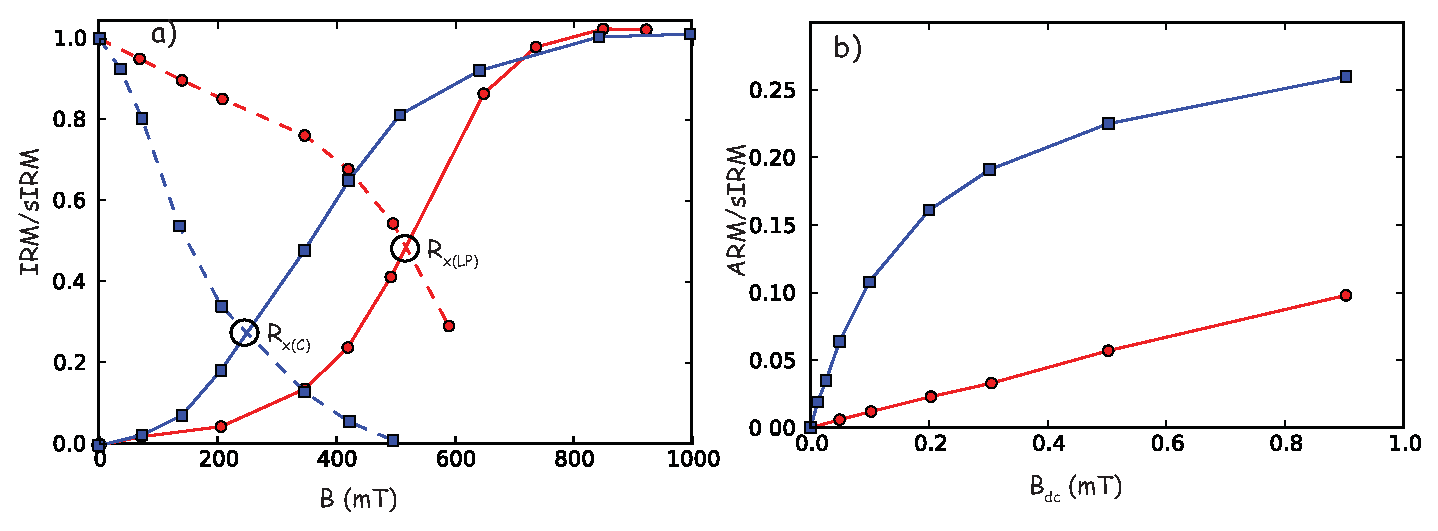
\includegraphics[width=14 cm]{EPSfiles/crossover.eps}
\caption{a) IRM acquisition (solid lines) versus progressive demagnetization of IRM with alternating fields (dashed lines) for two specimens.  Circles are the Lambert plagioclase (non-interacting uniaxial single domain magnetite particles) and squares are chiton teeth (interacting magnetite particles).  The field at which the demagnetization and acquisition curves cross (the cross-over point $R_x$) is sensitive to particle interaction.  [Data of Cisowski, 1981.]  b) ARM acquisition as a function of DC bias field for two specimens with different concentrations of magnetite.  The squares are for a low concentration of 2.6 x 10$^{-4}$ volume percent magnetite while the circles are for a high concentration of 2.33 volume percent.  [Data of Sugiura, 1979.]  }
\label{fig:crossover}
\end{figure}



\subsection{Magnetic interactions: IRM and ARM techniques}
\label{sect:interaction}


 \index{magnetization!remanent!isothermal!crossover}
Cisowski (1981) \nocite{cisowski81}  suggested that by comparing IRM acquisition curves like that shown in Figure~\ref{fig:irm} in Chapter 7 with the curves obtained by progressively demagnetizing the sIRM in alternating fields, one might be able to detect the effect of particle interaction.   He collected data from a specimen thought to be dominated by uniaxial single domain particles (the Lambert plagioclase) and from a specimen of chiton teeth, thought to be dominated by interacting particles of magnetite.   The IRM acquisition  data for the two specimens are shown as the solid lines in Figure~\ref{fig:crossover}a and the demagnetization of the saturation IRMs are shown as dashed lines.  The field at which the demagnetization curve crosses the acquisition curve is called the crossover point, here designated $R_x$.  This point should theoretically by reached when the IRM is half the saturation valued for uniaxial single domain particles.  The value of nearly 0.5 for the Lambert plagioglase ($R_{x(LP)}$ in Figure~\ref{fig:crossover}a) supports the claim of uniaxial single domain behavior for this specimen.  The much depressed value of $R_{x(C)}\simeq$ 0.25 for the chiton teeth  also supports the interpretation of significant inter-particle interaction for that specimen.  Magnetic interactions are nowadays more frequently assessed using the FORC diagrams discussed in Chapter 5, but the cross-over technique has been used extensively in the past.  

Another method for detecting magnetic interactions was developed by Sugiura (1979).   \nocite{sugiura79}  He showed that the ARM acquired as a function of DC bias field ($B_{DC}$) is a strong function of magnetite concentration.  We show examples of two ARM acquisition curves in Figure~\ref{fig:crossover}b, one with high magnetite concentration (2.33 volume percent, circles) and one with low magnetite concentration (2.5 x 10$^{-4}$ volume percent, squares).  The ARM acquisition curve for the low concentration  is highly non-linear and achieves a substantially higher fraction of the saturation IRM as opposed to the curve for the high concentration, which is linear and much less efficient.  


\begin{figure}[h!tb]
%\epsfxsize 9cm
%\centering \epsffile{EPSfiles/unmixing.eps}
\centering  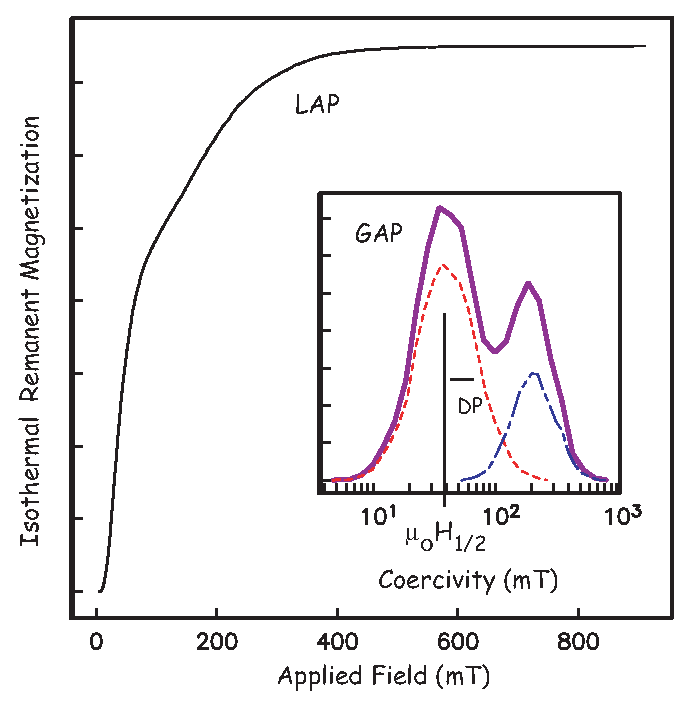
\includegraphics[width=9 cm]{EPSfiles/unmixing.eps}
\caption{Theoretical curve for the acquisition of IRM with two magnetic components with different coercivity spectra (see insert).  The acquisition curve can be differentiated to get the heavy solid line in the insert and then decomposed into the different components assuming some distribution of coercivity (in this case log-normal). The main plot is a ``linear acquisition plot'' (LAP) and the heavy solid line in the  inset is a ``gradient of acquisition plot'' (GAP) in the terminology of Kruiver et al. (2001).  $H_{1/2}$ and $DP$ are the fields required to magnetize half the population and the ``dispersion parameter'' of 
Robertson and France (1994) respectively.  Note that $H_{1/2}$ is a measure of  $H_{cr}  (H'''_{cr}$ in Table C.1)  if there is only one population of coercivities. }
\label{fig:unmixing}
\end{figure}
\nocite{robertson94} \nocite{kruiver01}

\subsection{IRM ``unmixing''}
\label{sect:unmixing}
\index{Robertson, D.J.}
\index{France, D.E.}\nocite{robertson94}
\index{isothermal remanenent magnetization!unmixing}
Robertson and France (1994)  suggested that if populations of magnetic materials have generally log-normally distributed coercivity spectra and if the IRM is the linear sum of all the contributing grains, then an IRM acquisition curve could be ``unmixed'' into the contributing components.  The basic idea is illustrated in Figure~\ref{fig:unmixing} whereby two components each with log normally distributed coercivity spectra (see dashed and dashed-dotted lines in the inset) create the IRM acquisition curve shown.  By obtaining a very well determined IRM acquisition plot (the ``linear acquisition plot'' or LAP in Figure~\ref{fig:unmixing} using the terminology of \nocite{kruiver01}
\index{Kruiver, P.}
Kruiver et al., 2001), one could first differentiate it   to get the ``gradient acquisition plot''  or GAP (heavy solid line in the inset to Figure~\ref{fig:unmixing}).   This then can be ``unmixed'' to get the parameters of the contributing components such as the mean and standard deviation of the log-normal distribution (called $B_{1/2}$ and $DP$ respectively by 
\index{Robertson, D.J.}
\index{France, D.E.}
Robertson and France, 1994).  For consistency with prior usage in this book, we use the $\mu_oH$ and $H$ terminology for coercivity depending on unit choice.   
  \index{coercivity!of remanence!estimation!$H_{1/2}$ method}
  Note that $H_{1/2}$ is a measure of  $H_{cr}$ if there is only one population of coercivities (see Table~\ref{tab:hystpars} and Appendix{app:hyst} for summary of coercivity of remanence).  Also,   unmixing of other  forms of magnetic remanence (e.g., ARM), demagnetization as well as acquisition, and other distributions are also possible as are  more complex methods of inversion  (see e.g.,
\index{Egli, R.}
 Egli, 2003).   \nocite{egli03}


\subsection{Combining thermal and isothermal information for rock magnetic characterization}


Another very useful technique for characterizing the magnetic mineralogy in a sample is the 
\index{isothermal remanenent magnetization!3D unblocking}
{\it 3D IRM  unblocking technique} of
\index{Lowrie, W.}
 Lowrie (1990). \nocite{lowrie90}
Some important magnetic phases in geological materials  (Table~\ref{tab:rockpars}; Chapter 6)
are magnetite
(maximum blocking temperature of $\sim$580$^{\circ}$C, maximum coercivity of about
0.3 T), hematite (maximum blocking temperature of 
$\sim$ 675$^{\circ}$C and maximum
coercivity larger than several tesla), goethite (maximum blocking temperature of
$\sim$ 125$^{\circ}$C and maximum coercivity of  much larger than 5 T), and
various sulfides.  The relative importance of these minerals in 
bulk samples can be constrained by  a simple trick that exploits
 both differences in
coercivity and unblocking temperature
\index{Lowrie, W.}
 (Lowrie, 1990).  
 
 This technique anticipates somewhat the chapter on demagnetization techniques.  It also should remind you of Problem 2 in Chapter 6.   In order to partially demagnetize a fraction of the magnetic remanence, a specimen is heated to a given temperature $T_i$ at which all those grains whose blocking temperatures have been exceeded are by definition superparamagnetic.  If the heating is done in zero applied field, the net magnetization of those grains will average to zero (because the SP particles are in equilibrium with a null field).  Therefore, the contribution of those grains with a blocking temperature of $T_i$ will be erased.   


\begin{figure}[htb]
%\epsfxsize 10cm
%\centering \epsffile{EPSfiles/3dirm.eps}
\centering  \includegraphics[width=10 cm]{EPSfiles/3dirm.eps}
\caption{a) Acquisition of IRM ($M_r$).  After applying a field of 2 T, the
specimen was subjected to two additional IRMs: 0.4 T and 0.12 T along
orthogonal axes.  b) Thermal demagnetization of a 3-axis IRM.  Each
component is plotted separately. [Figure from Tauxe, 1998.] }
\label{fig:3dirm}
\end{figure}
\nocite{tauxe98}

The ``3D IRM''  technique of Lowrie (1990) \nocite{lowrie90} proceeds as follows:

\begin{enumerate}
\item Apply an IRM along three orthogonal directions in three different
fields.  The  first field, applied along $\X_1$,
 should be sufficient to saturate all the
minerals within the specimen and is usually the largest field
achievable in the laboratory (say 2 T).  The second field, applied
along $\X_2$,  should be
sufficient to saturate magnetite, but not to realign high
coercivity phases, such as goethite or fine-grained hematite (say 0.4
T). The third IRM, applied along $\X_3$, 
should target low coercivity minerals and the
field chosen is typically something like 0.12 T.   

\item The composite magnetization can be characterized by determining
the blocking temperature spectra for each component.   This is done by
heating the specimen in zero field to successively larger temperatures, cooling then measuring the remaining
magnetization.  The magnitude of  
the three cartesian  components ($x_1, x_2, x_3$) of the remaining remanence is then plotted versus demagnetizing temperature.
\end{enumerate}


An example of 3D IRM data are shown in Figure~\ref{fig:3dirm}.
 The curve is dominated by a mineral
with a maximum blocking temperature of between 550$^\circ$ and 600$^{\circ}$C and has a
coercivity less than 0.12 T. These properties 
are typical
of magnetite (Table~\ref{tab:rockpars}; Chapter 6).  There is a small  fraction 
of a high coercivity ($>$0.4 T) 
mineral with a maximum unblocking temperature $>$ 650$^{\circ}$C,
which is consistent with the presence of hematite (Table~\ref{tab:rockpars}; Chapter 6).  








\section{Hysteresis parameters}
\label{sect:hyst}

IRM and ARM acquisition and demagnetization curves  can be a fecund source of information about the magnetic phases in rocks.  However, these are extremely time consuming to measure taking hours for each one.  Hysteresis loops on the other hand are quick, taking about 10 minutes to measure the outer loop.    In principle,  some of the same information could be obtained from  hysteresis loops as from  the IRM acquisition curves.   [For computational details, see Appendix~\ref{app:hyst}.]  

\subsection{The building blocks of hysteresis loops}

\index{hysteresis!loops}
Hysteresis loops, like IRM acquisition curves are the sum of all the contributing particles in the specimen.  There are several basic types of loops which are recognized as  the ``building blocks'' of the hysteresis loops we measure on geological materials.  
We illustrate some of  the building blocks  of possible hysteresis
loops in Figure~\ref{fig:bblocks}. Figure~\ref{fig:bblocks}a shows the negative slope typical of 
diamagnetic material such as carbonate or
quartz, while Figure~\ref{fig:bblocks}b shows a paramagnetic slope.  Such
slopes are common when the specimen has little ferromagnetic material and
is rich in  iron-bearing phases such as biotite or clay minerals.

 
\begin{figure}[h!tb]
%\epsfxsize 14.5cm
%\centering \epsffile{EPSfiles/bblocks.eps}
\centering  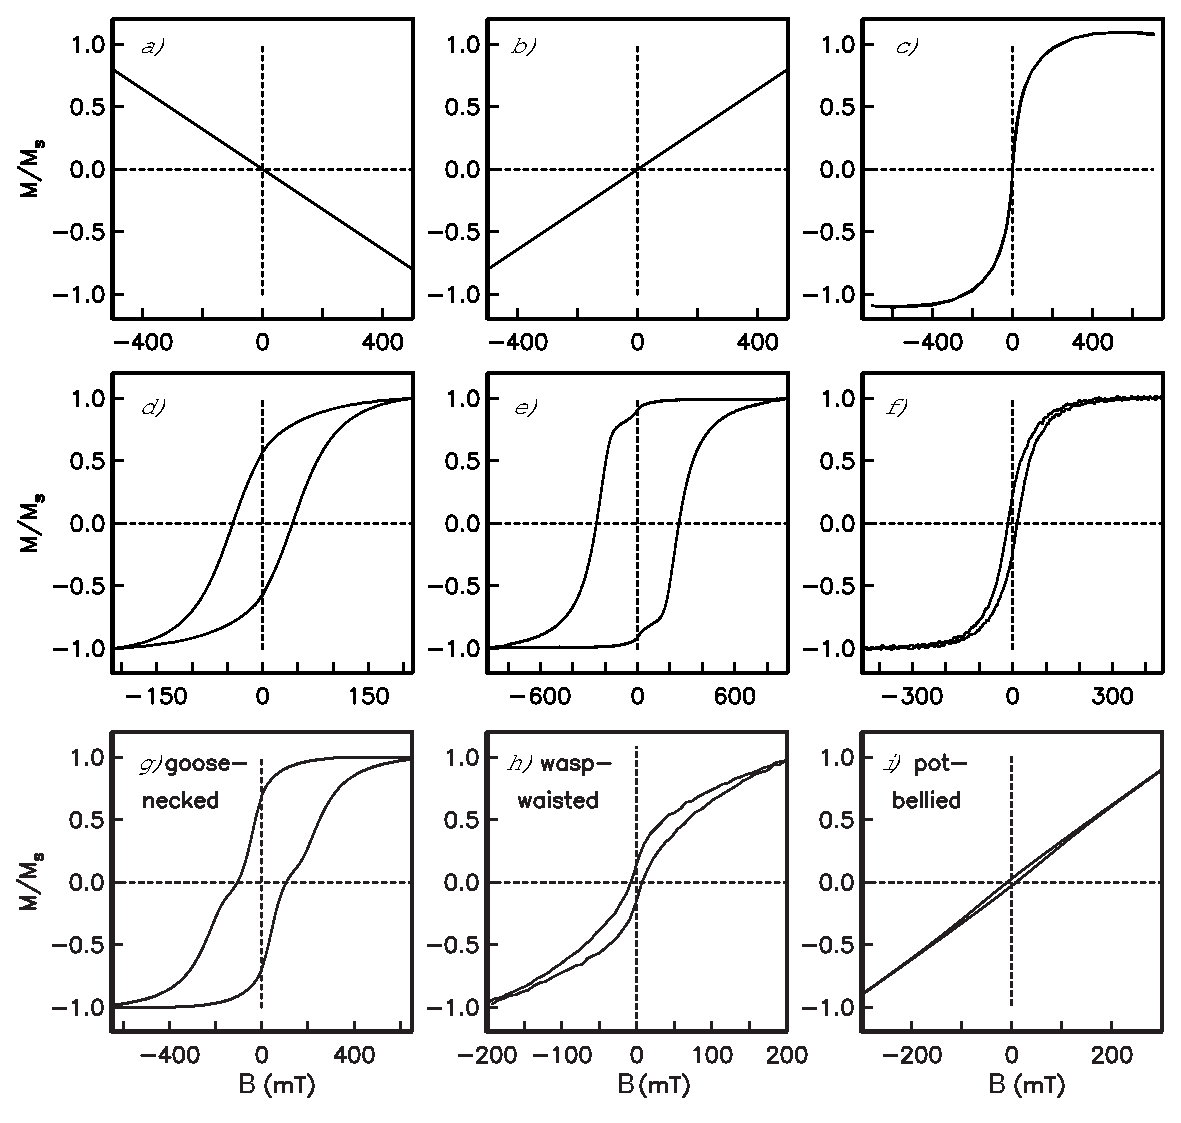
\includegraphics[width=14.5 cm]{EPSfiles/bblocks.eps}
\caption{Hysteresis loops of end-member behaviors: a)
diamagnetic, b) paramagnetic, c) superparamagnetic (data
for  submarine basaltic glass), d)
uniaxial, single domain, e) magnetocrystalline, single
domain, f) ``pseudo-single domain''. Hysteresis behavior of various mixtures:
g) magnetite, and hematite, h)
SD/SP magnetite (data from 
Tauxe et al.  1996), i) another example of SD/SP magnetite with a finer grained SP distribution.  [Figures redrawn from Tauxe, 1998.]}
\label{fig:bblocks}
\end{figure}\nocite{tauxe96b}
%\clearpage



When grain sizes are very small ($\sim$10 nm), a specimen
can display superparamagnetic ``hysteresis'' behavior
(Figure~\ref{fig:bblocks}c).  The SP curve follows a 
Langevin function $L(\gamma)$ (see Chapter 5) where $\gamma$ is
$M_svB/kT$, but integrates over the distribution of $v$ in the specimen.   



Above some critical volume, grains will have relaxation times that are
sufficient
to retain a stable remanence (Chpater 7).   Populations of  randomly oriented stable grains can produce hysteresis
loops with a variety of
shapes (see Chapter 5), depending on the origin of magnetic anisotropy and domain state.
We show loops from specimens that illustrate representative
styles of hysteresis behavior in Figure~\ref{fig:bblocks}d-f.  
Figure~\ref{fig:bblocks}d shows a loop characteristic of specimens whose
remanence stems from SD magnetite with uniaxial anisotropy.  In
Figure~\ref{fig:bblocks}e, we show data from specular hematite whose
anisotropy ought to be  magnetocrystalline in origin (hexagonal within the basal
plane).  Note the very high $M_r/M_s$ ratio of nearly one.  
 Finally, we show a loop 
that has lower $M_r/M_s$ ratios than single domain, yet some stability.  Loops of this type have been characterized as {\it pseudo-single domain}
 or PSD (Figure~\ref{fig:bblocks}f).  


\begin{figure}[htb]
%\epsfxsize 14.5cm
%\centering \epsffile{EPSfiles/interp.eps}
\centering  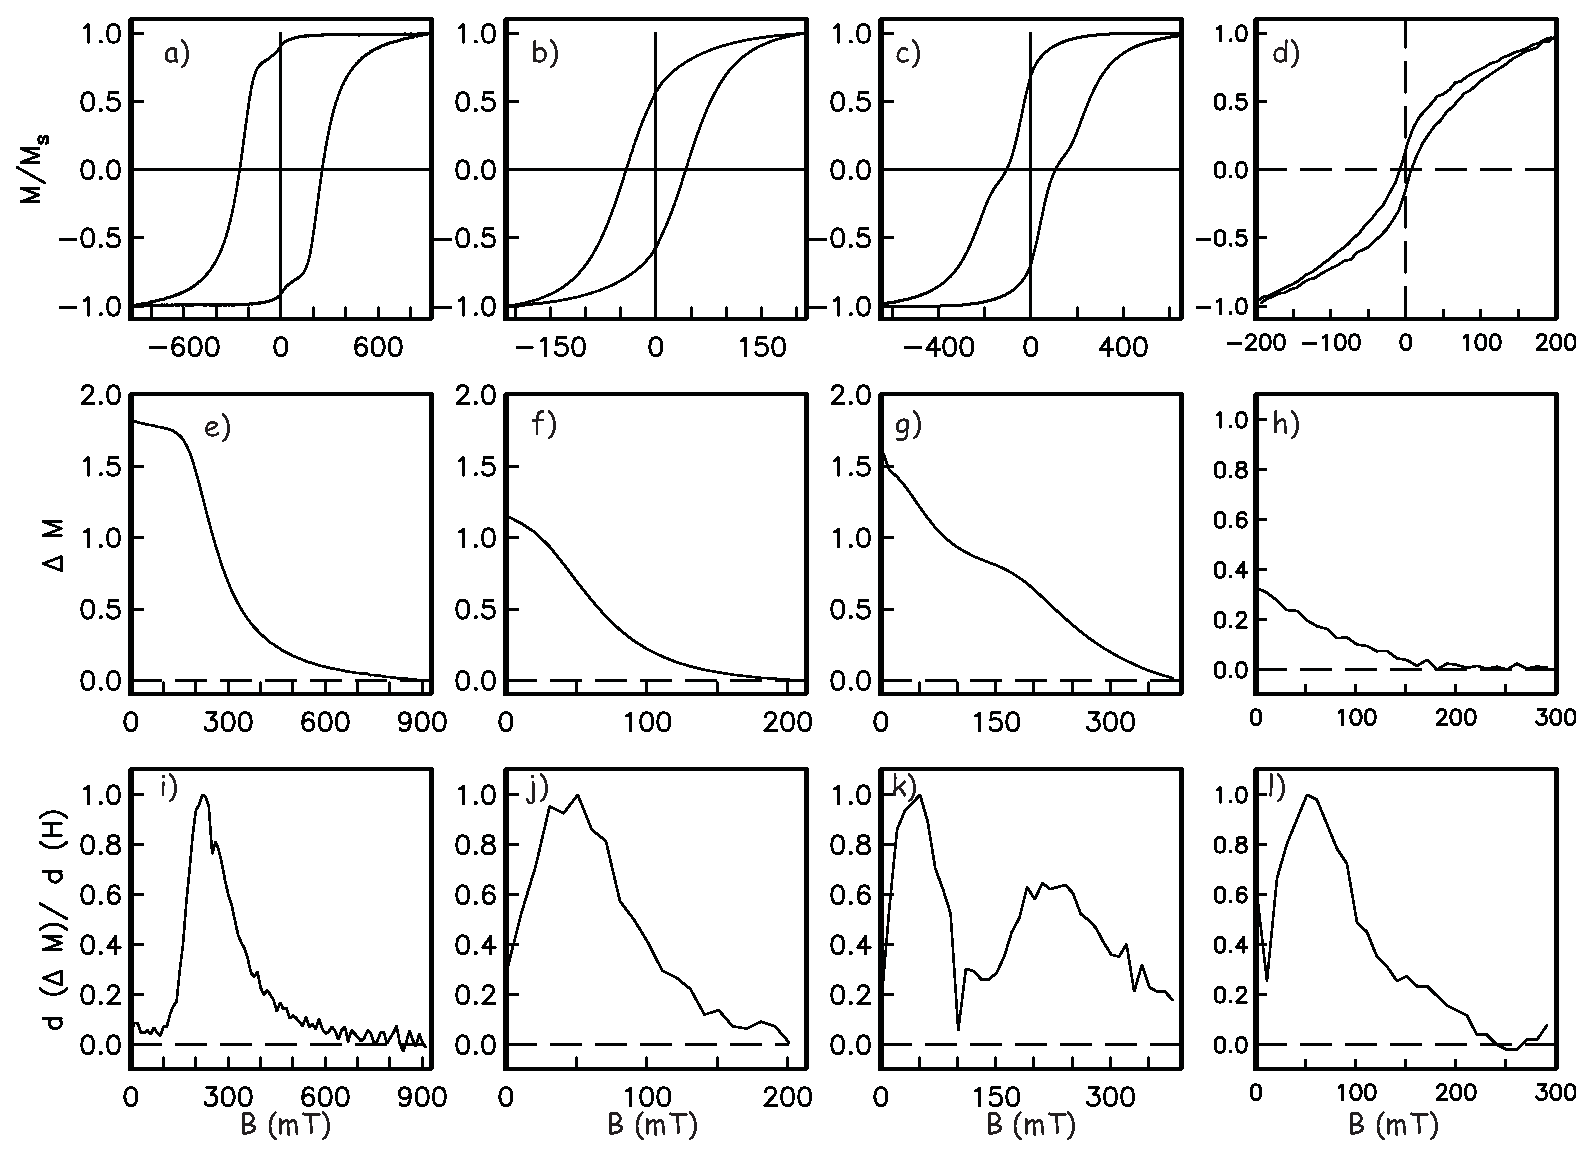
\includegraphics[width=14.5 cm]{EPSfiles/interp.eps}
\caption{ a-d) Hysteresis curves, e-h: $\Delta M$
curves and i-l) $d\Delta M/dH$ curves. Columns from the left to right:
hematite, SD magnetite, hematite plus magnetite, and SD plus SP
magnetite.  [Redrawn from Tauxe, 1998.]}
\label{fig:interp}
\end{figure}
\nocite{tauxe98}

\subsection {Hysteresis behavior of mixtures}

In the messy reality of geological materials, we often encounter
mixtures of several magnetic phases and/or domain states.  Such mixtures
can lead to distorted loops, such as those shown in
Figure~\ref{fig:bblocks}g-i.  In Figure~\ref{fig:bblocks}g, we show a
mixture of hematite plus SD-magnetite.  The loop is distorted in a
manner that we refer to as
{\it goose-necked}.  Another commonly observed mixture is SD plus SP
magnetite  which can result in loops that are
either 
{\it wasp-waisted} (see Figure~\ref{fig:bblocks}h) or 
{\it pot-bellied} (see Figure~\ref{fig:bblocks}i). 

Considering the loops shown in Figure~\ref{fig:bblocks}g-i, we immediately
notice that there are two distinct causes of loop distortion: mixing two
phases with different coercivities  and mixing SD and SP domain states.  Tauxe et al. (1996)  differentiated the two types of distortion
 as ``goose-necked'' and ``wasp-waisted'' (see
Figure~\ref{fig:bblocks}g,h) because they look different and they mean 
different things.    

\index{Jackson, M.J.}\nocite{jackson90} 
Jackson et al. (1990) suggested that the
\index{coercivity!of remanence!estimation!$\Delta M$ method}
 $\Delta M$ curve (see Figure~\ref{fig:sdloops}b in Chapter 5) could be differentiated to reveal different coercivity spectra contained in the hysteresis loop.   The $\Delta  M $ curve and its derivative ($d\Delta M/dH$) are sensitive only to the remanence
carrying phases, and not, for example, to the 
SP fraction. We can use these curves to distinguish the two sources of
distortion.  Hence, in Figure~\ref{fig:interp}, we show several representative
loops, along with  the $\Delta M$ and
$d\Delta M/dH$ curves. 
Distortion resulting from two phases with different coercivities (e.g., hematite plus
magnetite or two distinct grain sizes of the same mineral) results in a ``two humped'' $d\Delta M/dH$ curve, whereas
wasp-waisting which results from mixtures of SD + SP populations have only
one ``hump''.

\section{Trends in parameters with grain size} 
\label{sect:trends}

One quest of  applied rock magnetism is a diagnostic set of measurements that will yield unambiguous grain size  information.   To this end, large amounts of rock magnetic data have been collected on a variety of minerals that have been graded according to size and mode of formation.  The most complete set of data are available for magnetite, as this is the most abundant crustal magnetic phase in the world.   There are three sources for magnetite typically used in these experiments:  natural crystals that have been crushed and sieved into grain size populations, crystals that were grown by a glass ceramic technique and crystals grown from hydrothermal solution.    In Figure~\ref{fig:trends}a-c we show a compilation of grain size dependence of coercive force, remanence ratio,  and  coercivity of remanence respectively.    There is a profound dependence not only on grain size, but on mode of  formation as well.  Crushed particles tend to have much higher coercivities and remanence ratios  than grown crystals, presumably because of the increased dislocation density which stabilizes domain walls due to a minimum in interaction energy between internal stress and magnetostriction constants of the mineral.    These abnormally high values disappear to a large extent when the particles are annealed at high temperature -- a procedure which allows the dislocations to ``relax'' away (see, e.g., 
\index{Dunlop, D.J.}
\index{\"Ozdemir, \"O.}
Dunlop and \"Ozdemir, 1997). \nocite{dunlop97}     The behavior of low-field magnetic susceptibility is shown in Figure~\ref{fig:trends}d.  There is no strong trend with grain size over the entire range of grain sizes from single domain to multi-domain magnetite.    However, 
as already mentioned, susceptibility is predicted to be sensitive to the SD/SP domain state transition.  

Grain size trends in ARM are shown in Figure~\ref{fig:trends}e.   ARM has been converted to what is known as the ``susceptibility of ARM'' or $\chi_{ARM}$ (see Chapter 7).  This is done by assuming that ARM is linearly related to the applied DC field  and calculating the ratio of ARM (in for example, units of Am$^{2}$ to the DC field  (usually 50-100$\mu$T).  To do this, the DC field units must first be converted to units of $H$ by dividing by $\mu_o$ and the ARM must be a volume normalized remanence in units of $M$.  Because $H$ and $M$ are both in units of Am$^{-1}$, $\chi_{ARM}$ is dimensionless.   The  trend in $\chi_{ARM}$ shown in Figure~\ref{fig:trends}e is very poorly constrained because ARM is also a strong function of concentration and the method by which the particles were prepared.  


\begin{figure}[h!tb]
%\epsfxsize 13cm
%\centering \epsffile{EPSfiles/trends.eps}
\centering  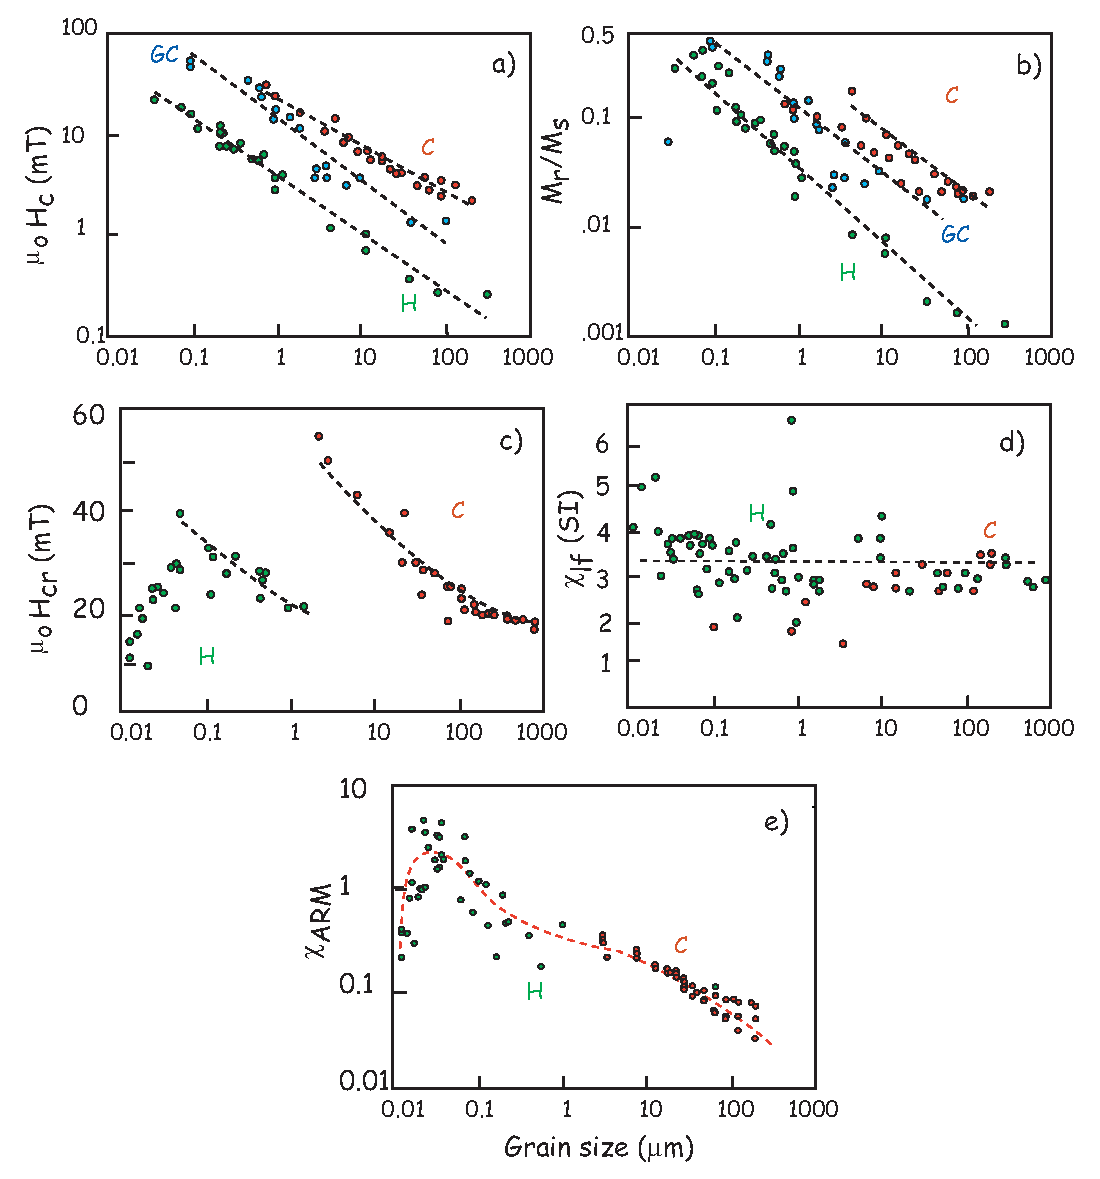
\includegraphics[width=13 cm]{EPSfiles/trends.eps}
\caption{ Grain size dependence in hysteresis parameters.  Crushed grains (red) indicated by ``C'',  glass ceramic grains (blue) indicated by GC; hydrothermal grains (green) indicated by ``H''.  a) Variation of coercivity ($\mu_oH_c$).  b) Variation of $M_r/M_s$. c) Variation of coercivity of remanence $\mu_oH_{cr}$. [Data compiled by Hunt et al., 1995.] d) Variation of susceptibility with grain size.  [Data compiled by Heider et al.,  1996.] e) Variation in $\chi_{ARM}$ with grain size.  [Data compiled by Dunlop and Argyle,  1997.]  }
\label{fig:trends}
\end{figure}

\nocite{heider96}\nocite{dunlop97b}


\begin{figure}[htb]
%\epsfxsize 13cm
%\centering \epsffile{EPSfiles/slag.eps}
\centering  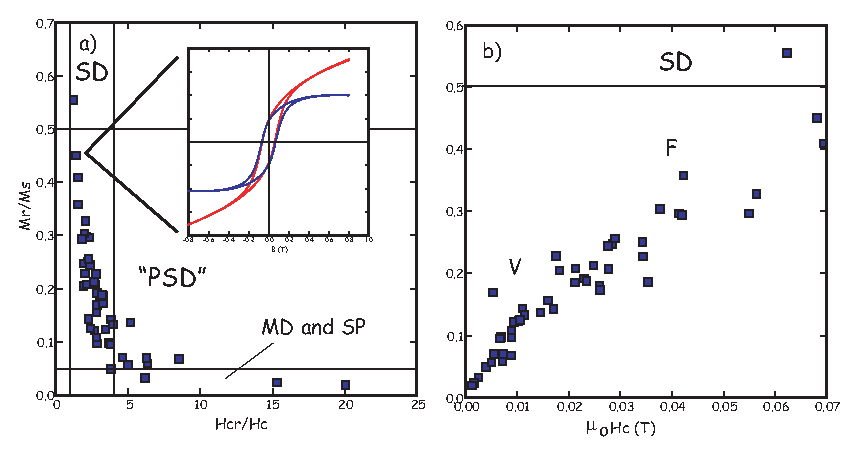
\includegraphics[width=13 cm]{EPSfiles/slag.eps}
\caption{Plots of hysteresis parameters from a collection of related specimens. a) Plot of $M_r/M_s$ versus $H_{cr}/H_c$.  Inset shows typical loop from which the ratios were derived.  b) Plot of $M_r/M_s$ versus $\mu_oH_c$.  [Data from Ben-Yosef et al., 2008.]}
\label{fig:slag}
\end{figure} \nocite{benyosef08}


\section{Ratios}
\label{sect:ratios}

A bewildering array of parameter ratios are in popular use in the applied rock and mineral magnetism literature.   The most commonly used ratios are listed in Table~\ref{tab:params}.    Most of these are new to us in this chapter and deserve some discussion.      Two of the most popular ratios are the hysteresis ratios $M_r/M_s$ and $H_{cr}/H_c$.   These are sensitive to remanence state (SP, SD, flower, vortex,  MD) and the source of magetic anisotropy (cubic,  uniaxial, defects), hence reveal something about grain size and shape.   Both of these ratios can be estimated from a typical hysteresis experiment (Chapter 5) and the results of many such experiments can be compiled onto a single diagram as in  Figure~\ref{fig:slag}.  

 Figure~\ref{fig:slag}a is known as the
 \index{Day, R.}
\index{diagrams!Day} \nocite{day77}
  {\it Day diagram} (Day et al. 1977; see Section~\ref{sect:mixtures} in Chapter 5).  Day diagrams are divided into regions of nominally SD, PSD and MD behavior using some theoretical bounds as guides.  The designation PSD stands for {\it pseudo-single domain} and has $M_r/M_s$ ratios in between those characteristic of SD behavior (0.5 or higher) and MD (0.05 or lower).  In practice  nearly all geological materials plot in the PSD box which comprises the entire flower and vortex state range. The PSD designation should really be split into the truly pseudo-single domain behavior of the flower state and what would better be described as {\it pseudo-multi-domain}  (PMD) behavior of the vortex state.    Nonetheless,    data such as those shown in Figure~\ref{fig:slag} are often interpreted in terms of grain size using the  crushed data shown in Figure~\ref{fig:trends} as calibration.  The problem arises however that the trends strongly depend on sample preparation and the absolute grain size interpretations are therefore usually wrong in the literature.  
 
 Part of the problem is that the hysteresis behavior of  multi-domain assemblages is similar to that of superparamagnetic particles (Chapter 5) and more information (such as behavior as a function of temperature) is necessary for a correct interpretation.  Moreover, by taking the ratio $H_{cr}/H_c$ we lose information.  For this reason, \nocite{tauxe02}
 \index{Tauxe, L.}
 Tauxe et al. (2002) argued for the much older practice of plotting $M_r/M_s$ versus $H_{cr}$ and $H_c$ separately 
 \index{N\'eel, L.}
 \nocite{neel55}
 (N\'eel, 1955).  This type of plot, known as the 
\index{diagrams!squareness-coercivity}
 squareness-coercivity diagram is shown in Figure~\ref{fig:slag}.  The ``F'' and ``V'' designations for flower and vortex respectively were approximated by micromagnetic modelling (Tauxe et al. 2002).   


\index{S-ratio}
The S-ratio is the ratio of the IRM acquired in a back field of  magnitude $x$ to the saturation IRM, $M_r$, (see Table~\ref{tab:params}).   
\index{HIRM}
$HIRM$ is not really a ratio, but  is the difference between the saturation IRM remaining after application of a backfield of magnitude $x$ and the sIRM (the fraction of $M_r$ ``harder'' than field $x$).   These parameters are frequently used in paleoceanographic and environmental applications because they are sensitive to changes in magnetic mineralogy.  

A ratio of saturation IRM to magnetic susceptibility ($M_r/\chi$ in Table~\ref{tab:params}) of greater than 20 kAm$^{-1}$ can indicate the presence of minerals other than magnetite (e.g, sulfides).   However,  identification of exactly which minerals is a rather complicated affair   (see 
\index{Maher, B.}
Maher et al., 1999).   \nocite{maher99}




Finally,  based on data similar to those shown in Figure~\ref{fig:trends},    \nocite{banerjee81}
\index{Banerjee, S.K.}
Banerjee et al.  (1981) argued that $\chi_{ARM}$ to $\chi$   can be used as a proxy for grain size changes in  magnetite (see e.g., Figure~\ref{fig:banerjee}).    
\index{King, J.}
King et al. (1982)  \nocite{king82}   went further  and suggested  specific grain sizes for a given ratio, but these were based partly  on crushed  magnetites whose behavior differs substantially from most naturally occurring magnetite.   Furthermore, as pointed out by 
\index{King, J.}\nocite{king83}
King et al. (1983), $\chi_{ARM}$ is a strong function of concentration, so  caution is warranted.  Finally,  the cgs units used in 
\index{King, J.}
King et al. (1982) have been translated into SI incorrectly in many applications (e.g., error in table in King et al., 1983).   Nonetheless, what is clear from Figure~\ref{fig:trends} is that susceptibility (away from the SP grain sizes) is virtually independent of grain size while $\chi_{ARM}$ is a strong function of grain size, so changes in $\chi_{ARM}$ normalized by $\chi_{lf}$ should in fact reflect changes in grain size.   


Three other ratios are listed in Table~\ref{tab:params},  ARM/$M_r$, and the two \nocite{koenigsberger38}
\index{K\"onigsberger, J.G.}
\index{K\"onigsberger ratios}
K\"onigsberger (1938) ratios $Q_n,Q_t$.     \nocite{maher99,koenigsberger38}
\index{Maher, B.}
Maher et al. (1999) suggest that the former be used to characterize particle interactions because particle interaction suppresses ARM acquisition, but not IRM acquisition.  The first K\"onigsberger ratio is  the ratio of the induced magnetization to remanent magnetization in a given field, a parameter useful for interpreting the origin of magnetic anomalies (whether from the rock's remanent magnetization or induced by the Earth's field).   The second is the ratio of the NRM (presumed to be thermal in origin) to a laboratory induced TRM.  This ratio is nowadays interpreted in terms of changes in the strength of the ancient magnetic field (to be discussed in later chapters), but
\index{K\"onigsberger, J.G.}
 K\"onigsberger himself believed the ratio to  reflect the age of the rock.   He envisioned a type of viscous decay of the remanence over time, so older rocks would have a lower value of $Q_t$ than younger ones, a trend that he observed in his own data spanning the last few hundred million years.   


\section{Applications of rock magnetism}
\subsection{Paleoclimatic information from lake sediments}


Although we have encountered numerous practical applications in this chapter already, there are 
many more.  Rock magnetic parameters are relatively quick and easy to measure, compared to geochemical, sedimentological and paleontological data.  When used judiciously, they can be enormously helpful in constraining a wide variety of climatic and environmental changes.  
There are three basic types of plots of the rock and mineral magnetic parameters discussed in this chapter:  maps,   bi-plots and depth plots.      

\begin{figure}[htb]
%\epsfxsize 7cm
%\centering \epsffile{EPSfiles/banerjee.eps}
\centering  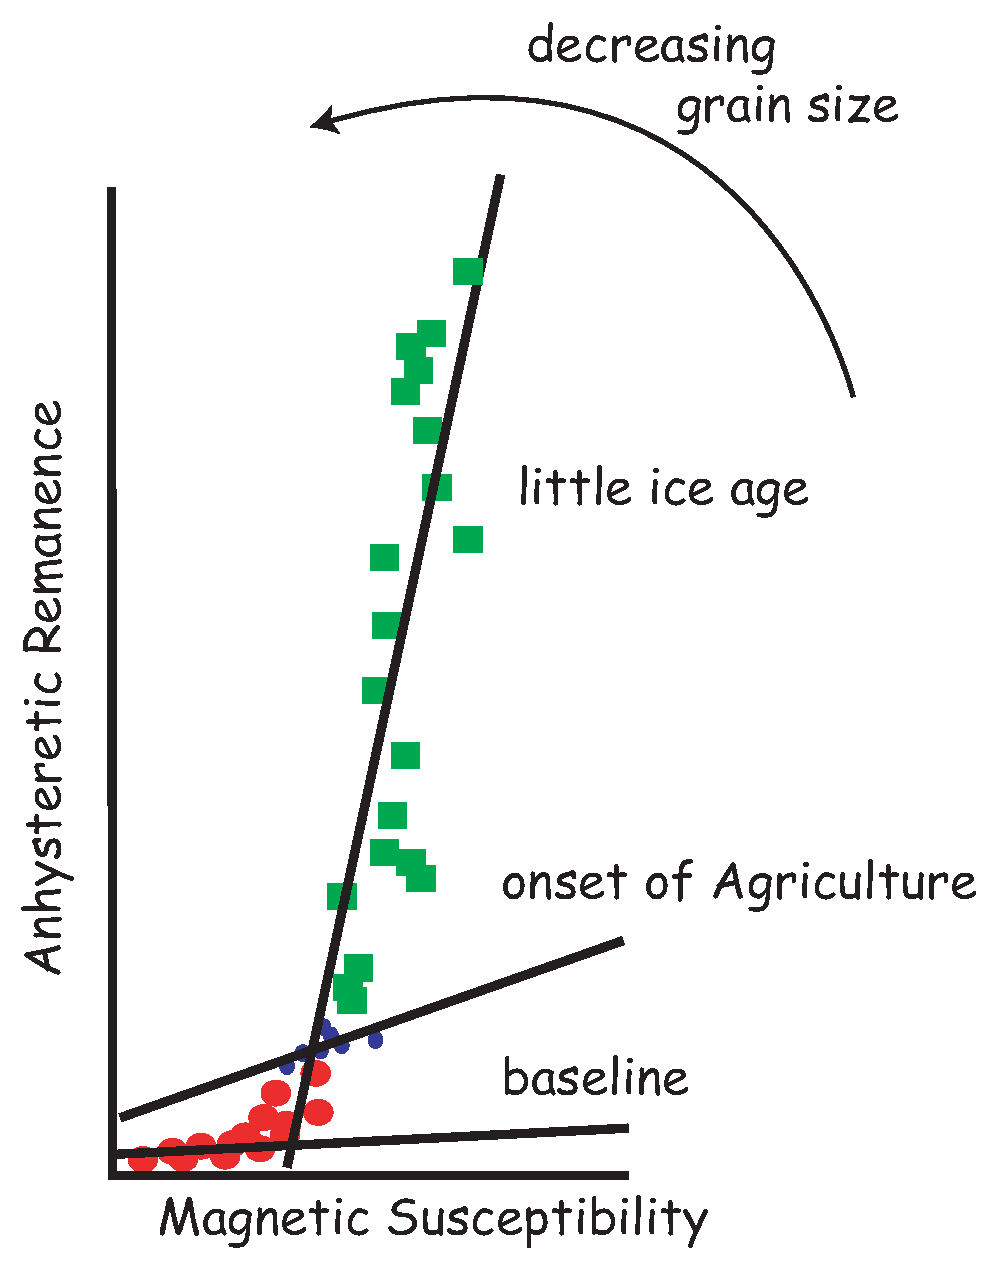
\includegraphics[width=7 cm]{EPSfiles/banerjee.eps}
\caption{Plot of ARM versus magnetic susceptibility for a core from Minnesota.  The different slopes are correlated with major climatic and anthropogenic events during the Holocene.  [Redrawn from Banerjee et al., 1981.]}
\label{fig:banerjee}
\end{figure} \nocite{banerjee81}


Because combustion related magnetic particles  (see, e.g.,  fly ash particle in Figure~\ref{fig:images}d), the extent  of anthropogenic pollution  can be visualized by mapping magnetic susceptibility.  
Biplots, for example ARM versus $\chi$ have been in use since 
 \nocite{banerjee81}
 \index{Banerjee, S.K.}
 Banerjee et al. (1981) (see e.g., Figure~\ref{fig:banerjee}).  They can be useful for detecting changes in grain size, concentration, mineralogy, etc.  If, for example, the data in a plot of $M_r$ versus  $\chi$ plot on a line, it may be appropriate to interpret the dominant control on the rock magnetic parameters as changes in concentration alone.

Depth plots are useful for core correlation,  variations in concentration, mineralogy and grain size as a function of depth.   An elegant example of the use of depth plots is the work of Rosenbaum et al. (1996).  \nocite{rosenbaum96}   Figure~\ref{fig:bucklake-1} shows depth variations of selected rock magnetic and major (Ti) and trace (Zr) element data along with the  pollen zones in sediment cores taken from Buck Lake, Oregon.  A simple (first order) interpretation of susceptibility would be that glacial (cold) and interglacial (warm) periods tapped different source areas in the drainage basin to deliver magnetite (higher susceptibility) and hematite (lower susceptibility) during different climatic periods. However, much more complexity emerges when (a) chemical analyses for concentration variation of certain key elements (Fe, Ti, Zr) and (b) petrographic observations of the magnetic fractions are considered. In Figure~\ref{fig:bucklake-2}a we observe that two elements, Ti and Zr, both derived from detrital heavy minerals are strongly correlated ($R^2$ = 0.82) and the regression line passing (nearly) through the origin confirms that neither element shows anomalous addition or subtraction.  In Figure~\ref{fig:bucklake-2}b and \ref{fig:bucklake-2}c,  Ti concentration is used as a measure of detrital input variations. Figure~\ref{fig:bucklake-2}b  shows that there has been post-depositional loss (vertical distance between the dashed and solid lines) of Fe, which is evidence that fluctuations in either iron or the magnetic parameters with depth cannot be a simple reflection of changes in detrital material delivery.


\begin{figure}[h!tb]
%\epsfxsize 14cm
%\centering \epsffile{EPSfiles/rosenbaum-1.eps}
\centering  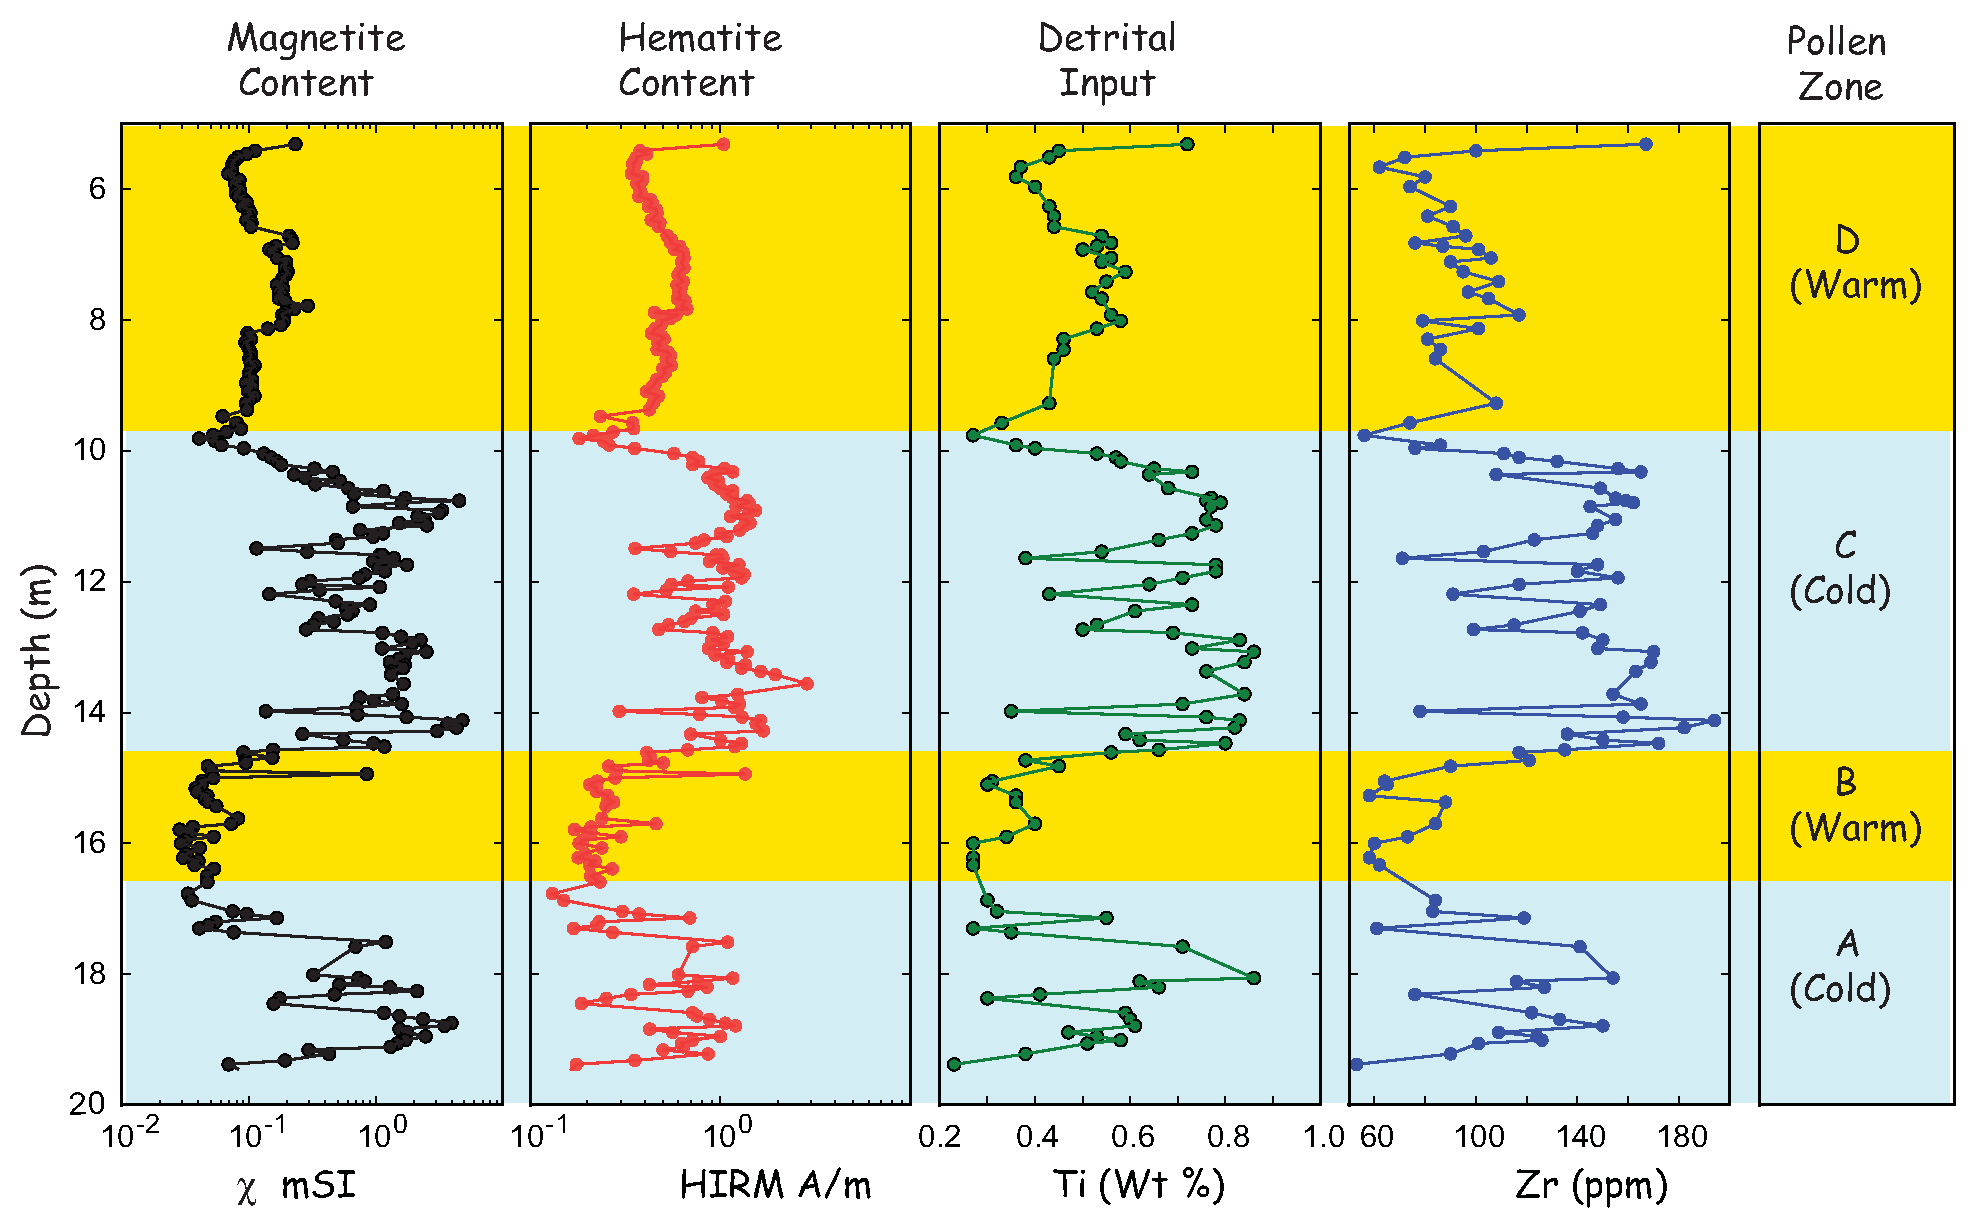
\includegraphics[width=14 cm]{EPSfiles/rosenbaum-1.eps}
\caption{Rock magnetic and trace element data  from Buck Lake [Data downloaded from \href{http://pubs.usgs.gov/of/1995/of95-673/of95-673.html}{http://pubs.usgs.gov/of/1995/of95-673/of95-673.html} and interpreted as in Rosenbaum et al., 1996].}
\label{fig:bucklake-1}
\end{figure}
\nocite{rosenbaum96}



In Figures~\ref{fig:bucklake-2}c and ~\ref{fig:bucklake-2}d, we get further information that hematite (proportional to HIRM) and magnetite (main contributor to susceptibility) both show negative intercepts when plotted against Ti. In both plots, HIRM and $\chi$ corresponding to the higher values of Ti are scattered, generally suggesting wide variations in detrital input, perhaps reflecting true changes in the types of detrital material delivered at different times.


But petrographic observations showed that the specimens with high scatter in HIRM (hematite) and $\chi$ (magnetite) contain fresh, relatively unweathered volcanic fragments with a wide variation of hematite and magnetite grains reflecting heterogeneity at source (volcano). Other samples of hematite and magnetite show pitting and evidence of wholesale mineral dissolution coinciding with offsets observed in HIRM and $\chi$. Taken together, the data from Figure~\ref{fig:bucklake-2} and petrographic evidence provide a more nuanced understanding of the past climate record at Buck Lake. Although the pollen data could mean variations in the temperature alone (glacial/interglacial), magnetic analyses and petrographic observations lead us to a further climatic/environmental clue: sections with wide scatter in susceptibility are heterogeneous and have large chunks of fresh, unaltered material.  This was  deposited during rapid high velocity water flows in the drainage basin. While the hydrologic conditions were much different (low rainfall and iron dissolution), then both HIRM and $\chi$  values are offset from the ideal dashed lines going through the origin at 45$^{\circ}$ to either axis. The lesson for us is that a multiparameter investigation enriches our understanding based on environmental magnetic data alone, and can provide additional information.

\begin{figure}[h!tb]
%\epsfxsize 11cm
%\centering \epsffile{EPSfiles/rosenbaum-2.eps}
\centering  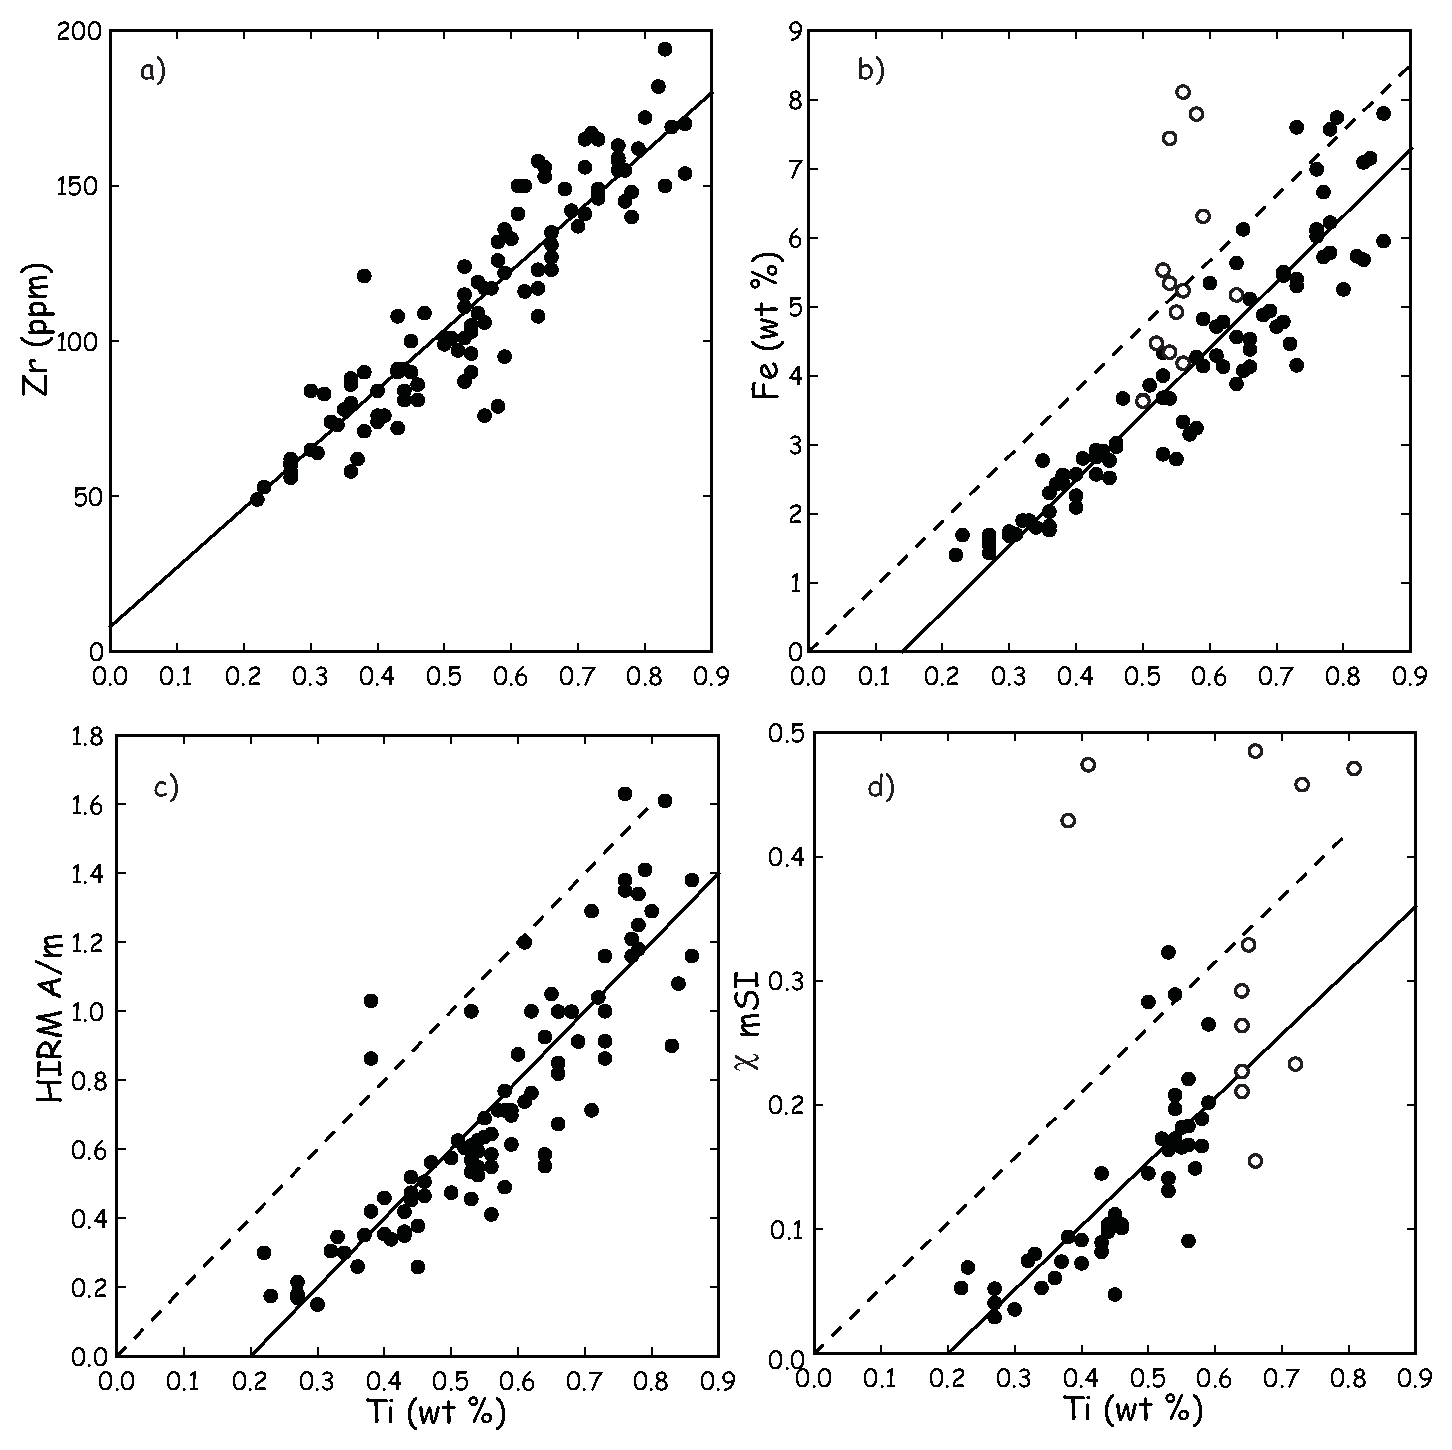
\includegraphics[width=11 cm]{EPSfiles/rosenbaum-2.eps}
\caption{Biplots of various trace elements and rock magnetic parameters. Solid lines are best-fit lines.  Dashed lines are theoretical lines with no Fe-loss.  Open symbols were excluded from best-fit line.  Note that many data are off the plot.   a) Zr against Ti.  b) Fe against Ti.  c) HIRM (hematite component) against Ti (proxy for detrital input).  d) $\chi$ (magnetite component) against Ti.   [Figures re-drawn from Rosenbaum et al. (1996) using data in Figure 8.15.]}  
\label{fig:bucklake-2}
\end{figure}




\subsection{Paramagnetic contributions to magnetic susceptibility}
\label{sect:rosenbaum}

Earlier in this chapter, we showed an early example 
\index{Banerjee, S.K.}
(Banerjee et al., 1981)\nocite{banerjee81}  of the utility of ARM-$\chi$ plots for detecting environmental and anthropogenic changes in a lake sediment archive. 
\index{King, J.}
King et al. (1982) \nocite{king82} rationalized such plots with $\chi_{ARM}$ on the y-axis instead of ARM so that  both axes are dimensionless. 
\index{Yamazaki, T.}
\index{Ioka, N.}
Yamazaki and Ioka (1997) \nocite{yamazaki97} %(Paleoceanography, 1997) 
used magnetic data from pelagic clay sediments to show that errors occur when the implicit assumption of identical sources contributing to x- and y-axis values breaks down.  In their pelagic clay sediments, as much as 25\% of the observed magnetic susceptibility ($\chi$) came from paramagnetic clays rather than iron oxides alone.






\begin{figure}[htb]
%\epsfxsize 14cm
%\centering \epsffile{EPSfiles/np21.eps}
\centering  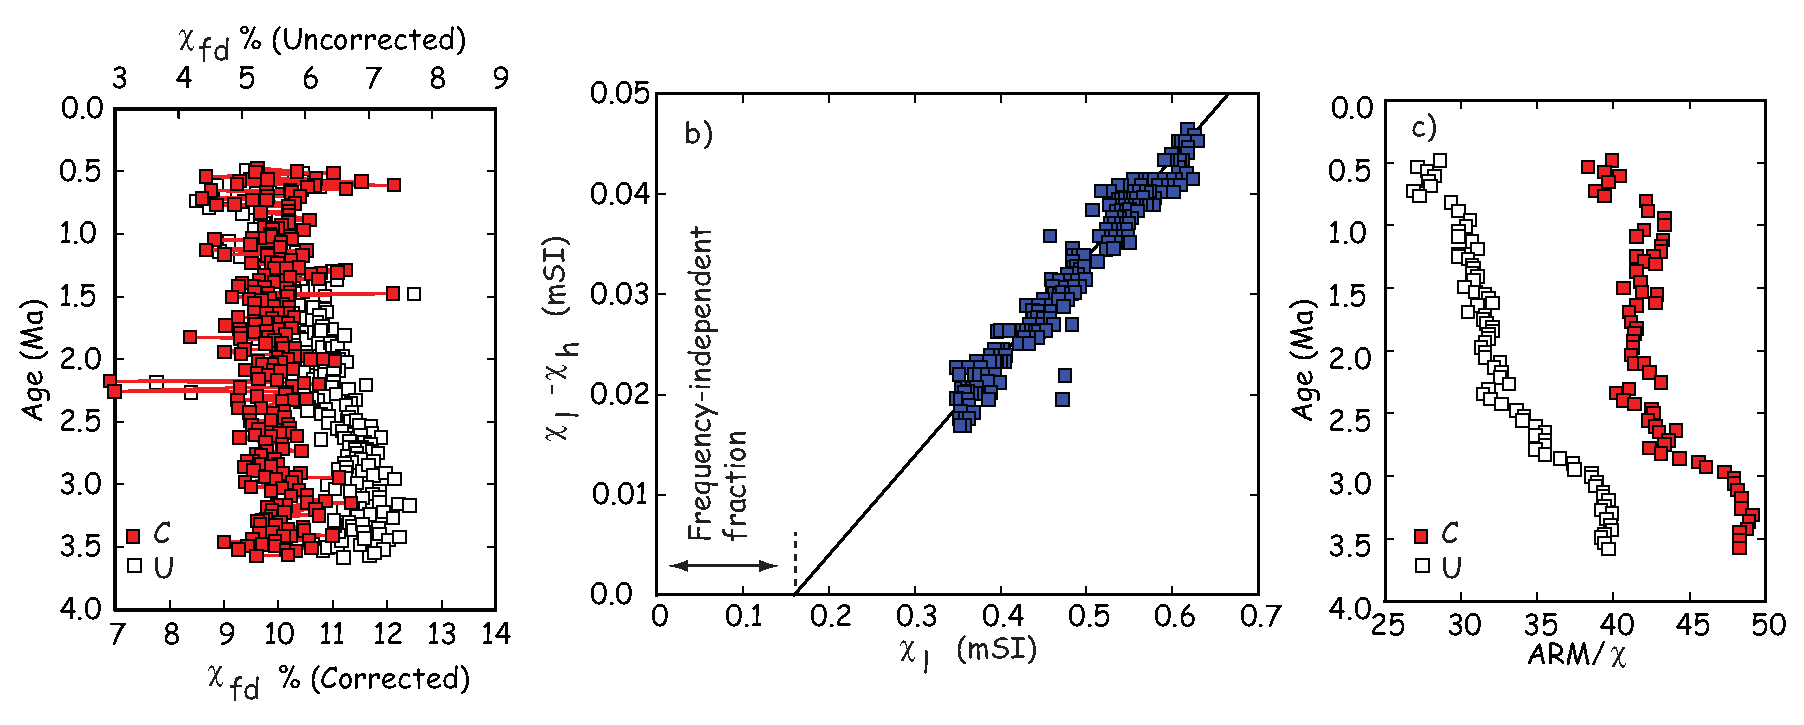
\includegraphics[width=14 cm]{EPSfiles/np21.eps}
\caption{a) Frequency dependence of magnetic susceptibility ($\chi_{fd}$) versus age for NP21, a pelagic clay core.   b)   Low-frequency magnetic susceptiblity ($\chi_{l}$) versus the difference between the low and high-frequency magnetic susceptibilities ($\chi_l-\chi_h$) for core NP21.  The value at the intersection of a linear regression line with the $\chi_l$ axis is interpreted as the frequency-independent fraction.     c)   Ratio of ARM to $\chi$ versus age for the uncorrected (U: open symbols) and corrected (C: solid symbols) data using the paramagnetic fraction of the susceptibility for core NP21.
[Data of  Yamazaki and Ioka, 1997.]}
\label{fig:yamazaki}
\end{figure}\nocite{yamazaki97}
Figure~\ref{fig:yamazaki}a shows two sets of frequency dependence of susceptibility measurements ($\chi_{fd}$).   In one (uncorrected) there is an increase from 10\% to 12\% with increasing age. This could be explained by a postulated increase in superparamagnetic (SP) particles at depth.  Frequency dependence is calculated by:

$$ \chi_{fd} ={ {\chi_{l} - \chi_{h}}\over {\chi_{l}}  }\cdot 100\%,$$

\noindent where $\chi_{l}$ and $\chi_h$ are the low and high frequency magnetic susceptibilities.   So the same frequency dependence would not result if $\chi_{l} $ had a frequency-independent contribution from paramagnetic clay.  In Figure~\ref{fig:yamazaki}b, the �corrected� values of $\chi_{l} $ are gotten by subtracting the paramagnetic or �high-field� susceptibility contributions ($\chi_{hf}$) obtained from the high field part of hysteresis loops (Chapter 5). As Figure~\ref{fig:yamazaki}a shows, the apparent increase in frequency dependence then disappears.

A similar error would occur if uncorrected $\chi_{l}$  values are used to derive the ratio ARM/$\chi_{l}$, which is inversely proportional to particle size (see Section~\ref{sect:trends}).  In Figure~\ref{fig:yamazaki}c where this ratio is plotted before and after high-field susceptibility correction, the slow variation between 1 and 2.8 Ma disappears, leaving a true increase in ARM/$\chi_{l} $ below 2.8 Ma and not at 1 Ma.

The parameters $\chi_{fd} $ (ultrafine or SP fraction) and ARM/$\chi_{l} $ (slightly larger single or pseudo-single domain fraction) are extensively used in paleoceanographic studies where contributions from paramagnetic clay can be substantial. For such ocean sediments, and some terrestrial sediments, a routine check for strong paramagnetism through high field susceptibility measurements is highly valuable.


\begin{figure}[htb]
%\centering \epsfxsize 14.5cm \epsffile{EPSfiles/jackson-1.eps}
 \centering 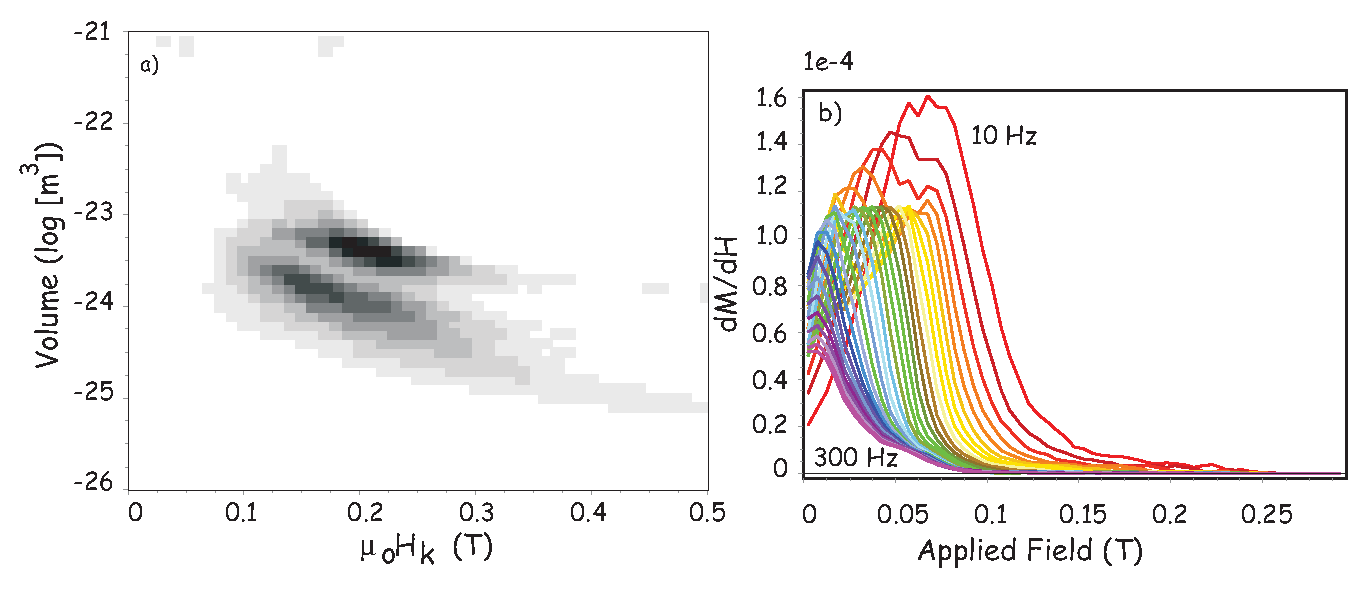
\includegraphics[width=11.5 cm]{EPSfiles/jackson-1.eps}
\caption{ a) Calculated grain distribution for the mixture of two Tiva Canyon Tuff specimens with different mean grain sizes and aspect ratios (contour interval = f$_{max}$/10). b) Calculated back-field spectra. [Redrawn from Figure 18 in  Jackson et al. 2006.]}
\label{fig:jackson-1}
\end{figure}\nocite{jackson06} 



\subsection{Separation of two superparamagnetic particle size distributions}

Particle sizes below 20-30 nm for magnetite are superparamagnetic at 300 K. Conventionally, parameters such as frequency dependence of susceptibility ($\chi_{fd} $) measure the relative amount of the SP particles and can distinguish them from thermally stable and larger single domain, pseudo-single domain and multidomain particles in a natural mixture, for example, loess/paleosol. However, we have recently seen that sometimes there is valuable information to be gleaned from identifiable mixtures of two modes of SP size distributions. In environmental magnetism studies, such mixtures may represent records of two diagenetic or chemical change events, or of two types distinguished by their origin: biogenic and inorganic. 

\index{superparamagnetism}
Superparamagnetic or thermal relaxation time for  magnetization of a uniaxial particle is defined by 
\index{N\'eel!equation}
N\'eel's equation (see Chapter 7):

$$
\tau = {1\over C}  \exp( { {M_sv\mu_oH_{k}}\over{2kT}}).
$$


\noindent  The particle volume distribution $f(v)$ can be estimated if the distribution of microscopic coercivity, $f(H_{k}$), is independently known or its approximate form can be assumed. 
\index{Jackson, M.J.}
Jackson et al. (2006) \nocite{jackson06} have formulated a general method to determine the joint distribution $f(v, H_{k})$ when both thermally stable single domain (SD, at 300 K) and thermally unstable smaller particles (SP) are present in a mixure. The raw data for applying the method utilizes the low temperature dependence of back field  demagnetization curves of isothermal remanent magnetizations acquired at different back fields at 300 K. 
To reduce the large amount of data thus acquired, 
\index{Jackson, M.J.}
Jackson et al. (2006) apply a ``tomographic''	reconstruction method that results in $ f(v, H_{k})$.  These are plotted on a 
\index{diagrams!N\'eel!tomographic reconstruction}
{\it N\'eel diagram} as shown in Figure~\ref{fig:jackson-1}a  for a laboratory-prepared SP + SSD mixture  of titanomagnetites obtained from different heights in Tiva mountain volcanic tuff deposit 
\index{Schlinger, C.M.}
(Schlinger et al., 1991). \nocite{schlinger91} Note that
\index{diagrams!N\'eel}
\index{N\'eel, L.}
N\'eel diagrams (after N\'eel, 1949) \nocite{neel49} 
are similar to the $K-v$  diagrams of Chapter 7, but show volume against coercivity instead of  the magnetic anisotropy constant.    The modes of both size distributions are close to 10 nm and yet the size/coercivity clusters are easily discernible. Direct size variations from Transmission Electron Microscopy (TEM) \index{Schlinger, C.M.}   \nocite{schlinger91}
(Schlinger et al., 1991) confirm the thermal fluctuation tomographic distributions in Figure~\ref{fig:jackson-1}a. The advantage of the magnetic method over TEM determination lies in the speed of measurement and in deriving distributions that represent a much larger spread of sizes.  Theoretical $dM/dH$ curves for the tomographic reconstruction underscore the distinction between the two grain size modes and are shown in Figure~\ref{fig:jackson-1}b.   


Figure~\ref{fig:jackson-2} shows another N\'eel diagram  obtained this time for a natural paleosol specimen from the Chinese loess plateau where the derived, and much wider, volume (10-100 nm) and coercivities are consistent with continuous pedogenic particle formation over tens of thousands of years. As 
\index{Jackson, M.J.}
Jackson et al. (2006) point out, however, back field remanence demagnetization curves spread over $\sim$30 discrete values of temperature from 300 down to 10 K can take 4-6 hours and much liquid helium expenditure.



\begin{figure}[htb]
%\centering \epsfxsize 14.5cm \epsffile{EPSfiles/jackson-2.eps}
 \centering 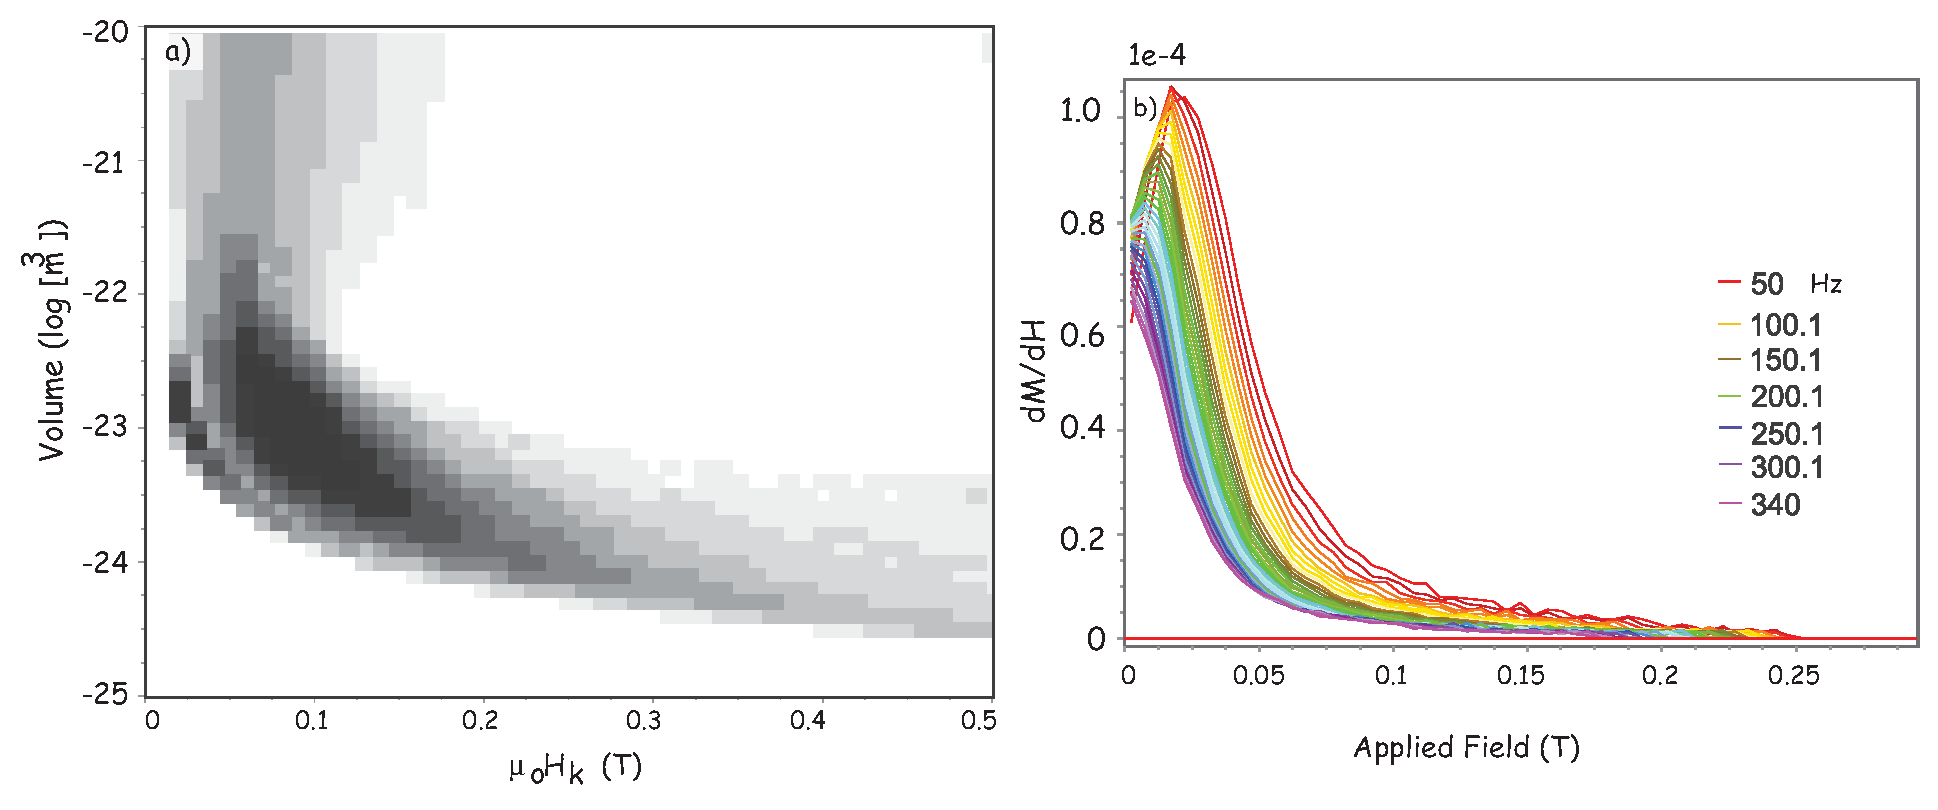
\includegraphics[width=14.5 cm]{EPSfiles/jackson-2.eps}
\caption{ a) Reconstructed grain distribution (contour interval of fmax/10) and b) best fit back-field spectra for a  paleosol specimen. The RMS misfit is $<5$\%. [Redrawn from Figure 21 in  Jackson et al. 2006.]}
\label{fig:jackson-2}
\end{figure}




\subsection{Identification of biogenic magnetite  in natural samples}
\label{sect:delta}

Here we provide a �real life� example of recognition of magnetite  produced by
\index{magnetotactic bacteria}
 magnetotactic bacteria in coastal pond sediments.   Magnetotactic bacteria  produce  chains of magnetic particles (see Chapter 6)  whose magnetocrystalline easy axes appear to be aligned.     
 \index{Moskowitz, B.M.}
 Moskowitz et al. (1993)  \nocite{moskowitz93}  developed a test   to detect the presence of aligned chains of magnetite.  
As was described in Chapter 4, magnetite undergoes a transition from cubic to monoclinic crystal structure as it cools through a temperature near 100-110 K known as the 
\index{Verwey transition}
Verwey transition temperature ($T_v$).    This transition results in a loss of magnetization (see Figure~\ref{fig:verwey} in Chapter 4).   This loss is quantified by:

\begin{equation}
\delta  = {  {M_{rs}(80) - M_{rs} (150)} \over {M_{rs} (80)} },
\label{eq:delta}
\end{equation}

\noindent where $M_{rs}$ is the saturation IRM remaining at 80 or 150 K while warming from $\sim$ 20 K.  
Specimens with intact chains of magnetite (magnetosomes) that are cooled from room temperature in the presence of a saturating field behave differently on warming through the Verwey transition than those cooled in low fields.   In other words,  the $\delta$ for field-cooled specimens ($\delta_{FC}$) is larger than that for low (essentially zero) field cooled specimens $\delta_{ZFC}$.    Extracted, and thus disturbed and disordered,  magnetosomes and inorganic SD and MD magnetites do not show a difference between $\delta_{FC}$ and $\delta_{ZFC}$.    
\index{Moskowitz, B.M.}
Moskowitz et al. (1993) \nocite{moskowitz93} explain this behavior by calling on intact magnetosomes to have [111] easy axes aligned  along the length of the chain.  
This makes the entire chain act as a uniaxial particle.   Near the Verwey transition is the isotropic point (see Figure~\ref{fig:K-T} in Chapter 4) at which the magnetocrystalline 
 anisotropy constant ($K_1$) goes through zero and the easy axis changes orientation from the [111] direction above it to the [100] below the isotropic point.  
 When intact magnetosomes  are cooled through $T_v$ 
in zero field, the new easy  axes are chosen at random from one of the three [100] directions.  When they cool through $T_v$ in a strong magnetic field, the [100] direction most closely aligned with the direction of the applied field will be chosen, instead of a random choice.  Therefore, the magnetization of these field cooled chains is not the sum of randomly selected [100] directions, but the sum of partially aligned [100] directions, hence the saturation remanence is enhanced relative to the random case.   Warming back through $T_v$, the ZFC curve joins the FC curve because both are warmed in the absence of a field.   Experimentally, the ratio of 
\index{paleomagnetic tests!$\delta-\delta$}
$\delta_{FC}/\delta_{ZFC}$ is about 2 for intact magnetosomes and nearly unity for extracted chains or inorganic magnetite.   This is known as the {\it $\delta-\delta$ test} for intact magnetosomes. 

\index{Moskowitz, B.M.}
Moskowitz et al.  (2008) applied the  $\delta-\delta$ test to  sediments from a salt water pond to locate the oxic-anoxic interface.  \nocite{moskowitz08} The presence of an oxic-anoxic interface (OAI) in lake waters and its environmental effects is usually discovered and studied using a combination of standard microbiological, geochemical and transmission electron microscopic techniques. Magnetic tests can be added to the tool-kit and have the  advantages   that  `bulk', i.e., unseparated material can be analyzed, they are highly sensitive, quick to make and are relatively inexpensive.    


\begin{figure}[htb]
%\epsfxsize 14cm
%\centering \epsffile{EPSfiles/moskowitz08-1.eps}
 \centering 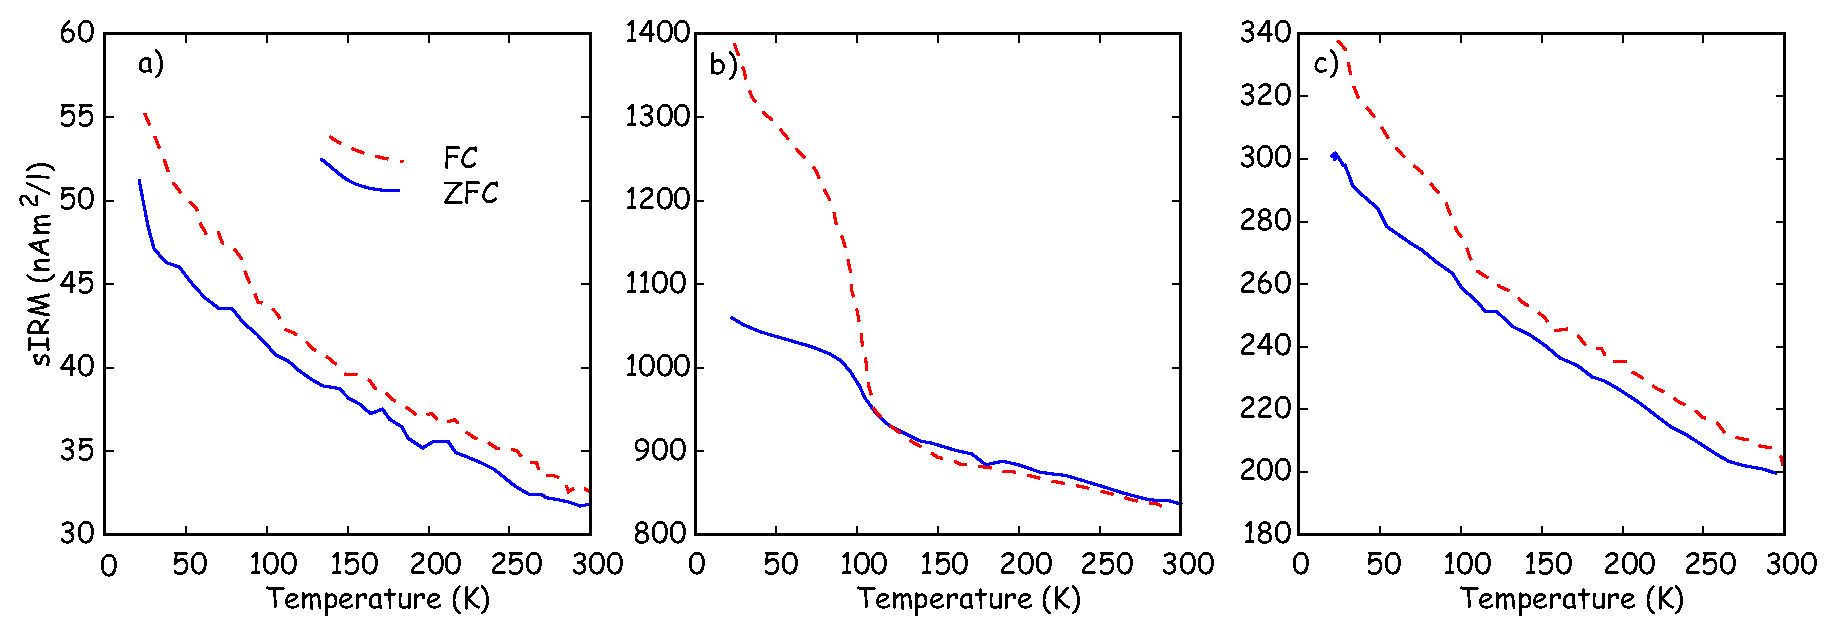
\includegraphics[width=14 cm]{EPSfiles/moskowitz08-1.eps}
\caption{Low-temperature FC (dashed line) and ZFC (solid line) demagnetization curves for selected water depths corresponding to a) above the oxic-anoxic interface (OAI;2.7 m), b)  bottom of OAI (3.5 m) , and c) below the OAI (4.0 m).   [Redrawn from Figure 9 in Moskowitz et al. (2008).]}
\label{fig:moskowitz-1}
\end{figure}



Moskowitz et al. (2008)  studied the  oxic-anoxic interface (OAI) in a salt water pond  in Falmouth, Masschusetts.  The OAI was between $\sim$3.1 m and $\sim$3.5 m below the sediment/water interface. Without knowing its exact location, water samples were collected from 2.5 m to 4.5 m depths and their solid contents filtered out for magnetic measurements. The immediate goal was to discover the presence of highest concentration of magnetite-producing magnetotactic bacteria that preferentially populate OAI. Magnetite (Fe$_3$O$_4$) has both ferric (Fe$^{3+}$) and ferrous  (Fe$^{2+}$) ions in its structure (see Chapter 3). Thus it is less common either in the fully oxic zone above OAI or in the fully anoxic zone (because of the presence of the reducing compound H$_2$S) below OAI.

\begin{figure}[htb]
%\epsfxsize 6cm
%\centering \epsffile{EPSfiles/moskowitz08-2.eps}
 \centering 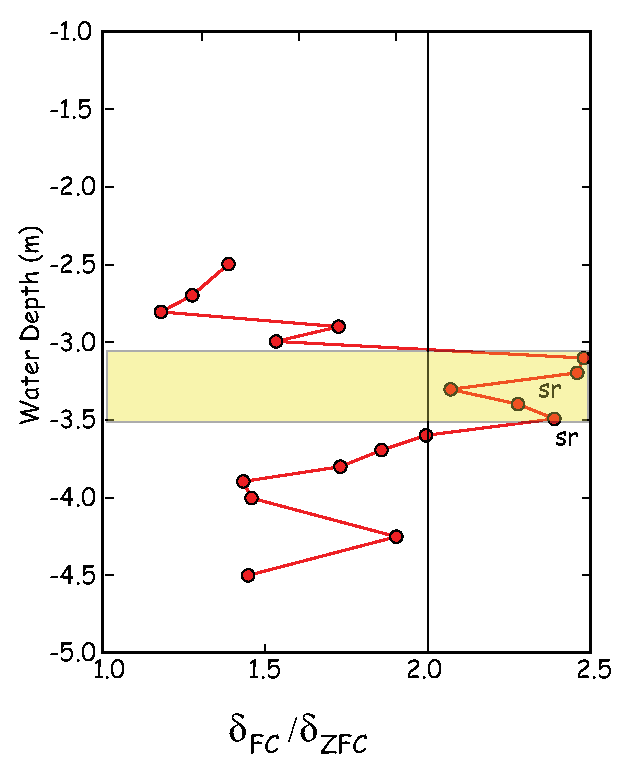
\includegraphics[width=6 cm]{EPSfiles/moskowitz08-2.eps}
\caption{$\delta_{FC}/\delta_{ZFC}$ ratios as a function of water depth. Shaded zone is the location of the
OAI based on chemical profiles.  sr:  short-rod shaped magnetotactic bacteria.   Values of $\delta_{FC}/\delta_{ZFC} > 2.0$  are characteristic of MMB and MRP bacteria  that have magnetite magnetosomes organized in chains. [Redrawn from Figure 10b in Moskowitz et al., 2008.]}
\label{fig:moskowitz-2}
\end{figure}



Figures~\ref{fig:moskowitz-1}a, b and c show the magnetic data acquired by warming from $\sim$15 K.  sIRM is applied  at this temperature to specimens initially cooled from 300 K using two different pre-treatments: the specimen is either  cooled in zero field (ZFC), or it is cooled in a large applied field (FC). The thermal demagnetization curves of specimens from above OAI (Figure~\ref{fig:moskowitz-1}a at 2.7 m) and below OAI (Figure~\ref{fig:moskowitz-1}c at 4.0 m) appear to be very similar. Both could be interpreted to contain a weak signature of the presence of very small amounts of magnetite in the form of small drops in sIRM around 95 K. However, the specimen shown in  Figure~\ref{fig:moskowitz-1}b from 3.5 m shows incontrovertible evidence for magnetite: the sharp drops in ZFC and FC sIRMs near the Verwey transition temperature. 

As defined earlier in this section, the magnitudes of the drops in sIRM can be expressed as $\delta_{FC}$ and $\delta_{ZFC}$.   Figure~\ref{fig:moskowitz-2} shows the depth variation of $\delta_{FC}/\delta_{ZFC}$ ratio which is known to be equal to 2.0 or higher for live bacteria with chains of magnetite magnetosomes inside (e.g.,
\index{Moskowitz, B.M.}
 Moskowitz et al. 1993). \nocite{moskowitz93}    As shown here, the ratio is 2.0 or higher for specimens within the chemically determined OAI (shaded zone). The symbol �sr� refers to short rod-shaped magnetite as discovered by electron microscopy. Taken together, the chemical and microscopic evidence help locate the extent of OAI, important for environmental condition study of this salt pond. But the $\delta_{FC}/\delta_{ZFC}$ ratio provides the same information, accurately and with speed, when the ratio rises above 2.0 in a given zone. The speed of analysis is crucial for environmental studies if one wants to survey the height variation of OAI at a dense network of points in the lake leading to information about organic productivity.

     


\section{Concluding remarks}

There are many other excellent examples of applications of rock magnetic data to solving thorny environmental problems.  Papers range from the highly useful to the frankly lunatic.  However, the field is alive and new imaginative and extremely clever applications are being published every month.  

\vskip .25 in\noindent SUPPLEMENTAL READINGS:Verosub and Roberts (1995).
 \nocite{verosub95}

\vskip 6pt

\section{Problems}

{\parindent 0pt \parskip 6pt 


\vskip -6pt
{\bf Problem 1}


a) Use the function {\bf ipmag.curie.} 
to calculate the Curie temperature of the data
contained in the two data files  {\it curie\_example.dat} and {\it curie\_example2.dat}  in the Chapter\_8 directory of the data  folder (see Preface instructions).    This funtion is designed to run in  a Jupyter notebook.

b) The way {\bf ipmag.curie}  works is to use a triangular sliding window and average over a range of temperature steps.   Then it calculates the first and second derivatives of the data and uses the maximum curvature (maximum in the second derivative) to estimate the Curie Temperature.   It can be tricky to get the ``right'' temperature, especially if there are two inflections and/or the data are noisy.  Therefore, the program will scan through a range of smoothing intervals. You can truncate the interval over which you want to look (see the help message for the {\bf ipmag.curie}) and set the smoothing interval.  
The program has a default smoothing window width of 3$^{\circ}$, which is usually too small to get an accurate Curie Temperature.  
The first data file is not very noisy and the second is noisier.   



 First  look at each data file using the defaults. Then, choose the optimal smoothing interval (the smallest
interval necessary
to isolate the correct peak in the second derivative). Finally, repeat
this, but  truncate
the data set to between 400$^{\circ}$ to 600$^{\circ}$.

  What is the Curie Temperature of the two specimens?   


{\bf Problem 2}

Rock magnetic parameters have been used extensively to study the Chinese sequences of loess.  Data from one such study (Hunt et al., 1995) \nocite{hunt95} is saved in the file loess\_rockmag.dat in the Chapter\_8 directory.   The data columns are:  stratigraphic position in meters below reference horizon,   total mass normalized magnetic susceptibility ($\kappa_{total}$) in ($\mu $m)$^3$kg$^{-1}$,   and sIRM in (mAm)$^2$kg$^{-1}$.   The paramagnetic susceptibility  ($\kappa_p$) for the section was relatively constant at about 60 nm$^3$kg$^{-1}$.   

Make plots of total susceptibility, ferromagnetic susceptibility ($\kappa_f = \kappa_{total} - \kappa_p$), sIRM and the ratio $\kappa_f/$sIRM/ versus stratigraphic position.     The reference horizon was the top of the modern soil, $S_0$.  

Magnetic susceptibility is closely linked to lithology, with peaks associated with soil horizons.  The triplet of peaks between about 20 and 27 meters are three units in soil $S_1$, which spans the interval 75 ka to 128 ka.  The material in between $S_0$ and $S_1$ is the top-most loess horizon $L_1$.  The interval below $S_1$ is $L_2$.    

 The explanation for the high magnetic susceptibility in the soils has been that there is magnetic enhancement caused by growth of superparamagnetic magnetite in the soil horizons.    Susceptibility, sIRM and their ratio have all  been used as magnetic proxies of past climate changes (mainly rainfall/year). But,  only one of them represents best the concentration of the superparamagnetic particle fraction created  from iron silicates by rainfall. Which of the profiles you plotted would be the best proxy for the superparamagnetic fraction and why?
 % use the IRM normalized susceptibitliy. Data from Hunt et al. 1995.
 }
 
 
 \begin{table}[h!tb]
 \begin{center}
\caption{Data for beach project.}
\label{tab:beach}
\begin{tabular}{ccc}
\hline
Specimen  &   $\chi$ (10$^{-5}$ SI)  &  Mass (gm) \\
\hline
\# 1 & 0.05 & 9.92\\
\# 2 & 0.2 & 10.00\\
\# 3 & 0.4 & 11.03 \\
\# 4 & 1.94 & 11.29 \\
\# 5 & 3.3 & 11.31 \\
\hline
\end{tabular}
\end{center}
\end{table}

 {\parindent 0pt \parskip 12pt 
 
 {\bf Problem 3}
 
 The sand on Scripps beach accumulates in the summer when gentle waves drop their load high up on the beach and erodes in the winter when high energy waves strip the sand away, leaving bare rock.  Sand accumulation and preservation therefore depends critically on density.  The sand can be crudely divided into a light colored fraction, composed of quartz, plagioclase, and feldspar and  a darker fraction, composed of  magnetite, pyroxene, amphibole, and biotite.    Wave action on the beach separates the sand into light and dark stripes with the darker sand being deposited at points when the water velocity slows down (over ripples or around stones, for example).     Average density measurements would help sedimentologists predict which beaches are more resistant to erosion during winter storms, but accurate density measurements are time consuming.   

As part of a class project,  students investigated whether magnetic susceptibility could be used as a proxy for density because it is much quicker and easier to measure.   Students collected  five test samples of sand ranging from light (\#1) to dark (\#5).  They dried and weighed out sand into 7 cc plastic boxes.    The specimens were measured on a Bartington susceptibility meter with units of 10$^{-5}$ SI, assuming a 10cc specimen.   
a)  Convert the susceptibility in Table~\ref{tab:beach}  (also in {\it beach\_sand.dat}  in the Chapter\_8 Datafiles folder)  into mass normalized units in m$^3$kg$^{-1}$.    Make plots of susceptibility against color (specimen number) and  density.   
b) Is there a relationship?  Pose a plausible hypothesis that explains your observations.   How would you test it?   

}



